\documentclass{ieeeaccess}
\usepackage{cite}
\usepackage{amsmath,amssymb,amsfonts}
\usepackage{algorithmic}
\usepackage{graphicx}
\usepackage{textcomp}
\usepackage{hyperref}
\usepackage[table]{xcolor}
\usepackage{algorithm}
\usepackage{algorithmic}
\usepackage{multirow}

\usepackage{bm}
\makeatletter
\AtBeginDocument{\DeclareMathVersion{bold}
\SetSymbolFont{operators}{bold}{T1}{times}{b}{n}
\SetSymbolFont{NewLetters}{bold}{T1}{times}{b}{it}
\SetMathAlphabet{\mathrm}{bold}{T1}{times}{b}{n}
\SetMathAlphabet{\mathit}{bold}{T1}{times}{b}{it}
\SetMathAlphabet{\mathbf}{bold}{T1}{times}{b}{n}
\SetMathAlphabet{\mathtt}{bold}{OT1}{pcr}{b}{n}
\SetSymbolFont{symbols}{bold}{OMS}{cmsy}{b}{n}
\renewcommand\boldmath{\@nomath\boldmath\mathversion{bold}}}
\makeatother

\def\BibTeX{{\rm B\kern-.05em{\sc i\kern-.025em b}\kern-.08em
    T\kern-.1667em\lower.7ex\hbox{E}\kern-.125emX}}

%Your document starts from here ___________________________________________________

\graphicspath{ {./images/} }

\begin{document}
\history{Date of publication xxxx 00, 0000, date of current version xxxx 00, 0000.}
\doi{10.1109/ACCESS.2024.0429000}

\title{Refining Software Clustering: The Impact of Code Co-Changes on Architectural Reconstruction}
\author{\uppercase{Adelina Diana Stana}\authorrefmark{1} and
\uppercase{Ioana Șora}\authorrefmark{2}
}

\address[1]{Department of Computer and Information Technology,
Politehnica University of Timisoara, Romania (e-mail: adelina.stana@cs.upt.ro)}
\address[2]{Department of Computer and Information Technology,
Politehnica University of Timisoara, Romania (e-mail: ioana.sora@cs.upt.ro)}

\markboth
{Author \headeretal: Preparation of Papers for IEEE TRANSACTIONS and JOURNALS}
{Author \headeretal: Preparation of Papers for IEEE TRANSACTIONS and JOURNALS}

\corresp{Corresponding author: Adelina Diana Stana  (e-mail: adelina.stana@cs.upt.ro).}

\begin{abstract}  
Version control systems are essential for tracking and managing changes in software code. They also provide information about the relationships between software entities: when multiple entities (e.g., classes or interfaces) are frequently modified together, it may indicate an underlying connection between them. These code co-changes can be analyzed to uncover logical dependencies — dependencies that complement structural or lexical dependencies.
While structural dependencies are extracted using code analysis techniques, logical dependencies can be extracted solely from version control system logs. This makes their extraction independent of the programming language.

Our work investigates filtering techniques to eliminate co-change situations that are not meaningful as logical dependencies. The effectiveness of these filtering techniques is investigated by using the obtained logical dependencies in architectural reconstruction, a reverse engineering activity aimed at recovering a system's modular structure.

This paper explores the use of logical dependencies as input for architectural reconstruction. The main goal is to investigate whether logical dependencies can complement or even fully replace structural dependencies in this process. We use clustering based on software dependencies to group related entities into modules.

We conduct experiments on four open-source Java projects using three clustering algorithms (Louvain, Leiden, and DBSCAN) and two evaluation metrics (Modularization Quality and MoJoFM). We consider three different dependency configurations: (1) only structural dependencies, (2) only logical dependencies, and (3) their combination. Our goal is to assess which configuration performs best and to examine the advantages and limitations of using logical dependencies.

\end{abstract}  

\begin{keywords}
Architectural reconstruction, code co-changes, logical dependencies, software clustering, software dependencies, versioning system.
\end{keywords}

\titlepgskip=-21pt

\maketitle

\section{Introduction}
\label{sec:introduction}

Software systems often lack sufficient or up-to-date documentation. Even if there was original documentation at the beginning of development, it may become outdated over the years. Additionally, the original developers may leave the company, taking with them knowledge about how the software was designed. This situation challenges the teams when it comes to maintenance or modernization. In this context, recovering the system's architecture is essential. Understanding the system's architecture helps developers evaluate better and understand the nature and impact of changes they must make. 

A common form of architectural abstraction involves identifying the system's modules. These modules represent the architectural components of the system and are created by grouping related software entities. Software entities are the fundamental building blocks of a program. Depending on the programming paradigm, they may include procedures and functions (in procedural programming) or classes and interfaces (in object-oriented programming). 


Software architecture reconstruction is very often a bottom-up process where higher-level architectural abstractions are built starting from low-level existing artifacts: most often source code representations, but also other kinds of information, such as dynamic information extracted from a system execution or historical data from version control system repositories \cite{ducassepollet}. If source code is used as input, a frequently used approach in state-of-the-art is to extract structural dependencies between the software entities through static analysis \cite{tzerpos1, wu, b10, bunch, b12, b19}. A few approaches \cite{acdc, b18} also use lexical dependencies (relationships between entities based on naming similarities and conventions).

Many state-of-the-art architectural reconstruction approaches use various software clustering techniques to process the different types of inputs. Software clustering involves creating cohesive groups (modules) of software entities based on their dependencies and interactions.

In this work, we focus on how to best exploit information from version control systems in the process of software clustering. Although previous works have used co-changes alone or together with other dependency types for software clustering \cite{b18, b16}, our goals are:
\begin{itemize}
  \item to investigate filtering techniques that make co-changes into more reliable logical dependencies
  \item to investigate the use of logical dependencies obtained from filtered co-changes in software clustering
\end{itemize}

The need to filter co-changes before considering them as logical dependencies stems from the observation that some entities may be accidentally updated together in the same commit. The more frequently they are updated together (they appear in more commits), the more likely it is that there is a dependency between them. Also, a commit of a large size (involving a large number of files) is most likely a belated commit, or it reflects unrelated updates (such as formatting or configuration updates).
The works of Zimmermann et al. \cite{Zimmermann:2004:MVH:998675.999460, b7} and  Capiluppi et al. \cite{b1, b12017} introduced the idea that co-changes must be filtered before considering them as dependencies. These works proposed different empirical filtering techniques. Also, the filtered logical dependencies have been used in other types of applications, not just software architecture reconstruction.

In our work, we use for filtering the metric of commit size and introduce a new metric called the connection strength metric. This metric is derived from the confidence metric introduced by Zimmermann et al. \cite{Zimmermann:2004:MVH:998675.999460} and used by other authors for various software engineering tasks \cite{article-Kagdi-commit}, \cite{Mandal-clones}. We introduced this new metric to alleviate some limitations of the confidence metric, as we explain in Section \ref{subsec:ld} of this paper. The connection strength metric was introduced in our previous research on using logical dependencies to improve key class detection \cite{b1}, \cite{b4}.

In this work, we refer to logical dependencies (LD) as being derived from co-changes after our filtering technique has been applied.

The following research questions guide our investigation:

\begin{itemize}
\item \textbf{RQ1:} Does using structural dependencies (SD) combined with logical dependencies (LD) improve software clustering results compared to traditional approaches that primarily rely on structural dependencies?
\item \textbf{RQ2:} Can using only logical dependencies (LD) produce good software clustering results?
\item \textbf{RQ3:} How do different filtering settings for logical dependencies (LD) impact clustering results, and which filtering settings provide the best performance?
\end{itemize}

To answer these research questions, we apply three different clustering algorithms (Louvain, Leiden, and DBSCAN) to different open-source projects. We then evaluate the results using two frequently used metrics in software clustering:  MQ (Modularization Quality) \cite{b10} and MoJoFM (Move and Join e\textbf{F}fectiveness \textbf{M}easure) \cite{mojofm}. We have chosen these two metrics to offer complementary insights, with each addressing the potential limitations of the other. Together, they allow us to assess the effectiveness of using structural and logical dependencies separately and in combination. The MoJoFM metric is used for external evaluation, evaluating against the perspective of the system's architect or developers. The MQ metric is used for internal evaluation based on the software structure itself. 


The main contributions of this paper are as follows:
\begin{itemize}
  \item We introduce a filtering approach that refines co-changes into reliable logical dependencies using two metrics: commit size and a confidence-based connection strength metric.
  \item We evaluate the impact of logical dependencies in software clustering, both alone and in combination with structural dependencies, using three clustering algorithms and two evaluation metrics (MQ and MoJoFM).
\end{itemize}

The paper is structured as follows. In Section \ref{sec:related_work}, we review the related work and previous studies that used various dependencies for software clustering and their metrics for evaluation.
Section \ref{sec:dependencies} provides an overview of structural and logical dependencies used in our approach, explaining how these dependencies are extracted.
Section \ref{sec:clustering_algorithms_evaluation} describes the clustering algorithms and evaluation metrics used, and Section~\ref{sec:tool_workflow} describes the tool implemented for this paper's experiments.
The plan of our experiments on four open-source projects is presented in Section \ref{sec:plan}. Sections \ref{sec:results} and \ref{sec:rq} present and evaluate our results using the Modularization Quality (MQ) metric and the MoJoFM metric. 
Finally, Section \ref{sec:conclusion} contains our conclusions and findings.

\subsection{Abbreviations and Acronyms}

The following abbreviations and acronyms are used throughout this article:

\begin{itemize}
    \item \textbf{LD}: Logical Dependencies
    \item \textbf{SD}: Structural Dependencies
    \item \textbf{MQ}: Modularization Quality
    \item \textbf{MoJoFM}: Move and Join Effectiveness Measure
\end{itemize}

\section{Related Work}
\label{sec:related_work}

Several studies have explored the use of different types of dependencies in software clustering, applying different algorithms to improve clustering results and using various metrics to evaluate the results obtained.

Tzerpos and Holt developed ACDC (Algorithm for Comprehension-Driven Clustering). This pattern-driven clustering algorithm uses subsystem structures such as source file patterns, directory patterns, system graph patterns, and support library patterns to detect similarities and create clusters \cite{acdc}. For result evaluation, the authors introduced the MoJo metric, which counts the minimum number of move and join operations required to transform one clustering result into another, assessing how close one clustering solution is to another \cite{b3}, \cite{tzerpos1}. Later, Wen and Tzerpos introduced the MoJoFM metric, an enhanced version of the original MoJo distance metric for more effective measurements, as presented in more detail in subsection \ref{subsec:mojofm} \cite{mojofm}.

Corazza et al. \cite{b13}, \cite{corazza2} used lexical dependencies derived from code comments, class names, attribute names, and parameter names, applying Hierarchical Agglomerative Clustering (HAC) to group-related entities. For evaluating the results, the authors used a metric based on the MoJo distance metric and NED (Non-Extremity Cluster Distribution), which measures that the formed clusters are not too large or too small.

Andritsos and Tzerpos ~\cite{tzerpos1} used structural dependencies and nonstructural attributes, such as file names and developer names, and proposed the LIMBO algorithm, a hierarchical clustering algorithm for clustering software systems. They used the MoJo distance metric to evaluate the algorithm's output.

Anquetil et al.~\cite{b14} also used lexical information, including file names, routine names, included files, and comments. They applied an n-gram-based clustering approach to detect semantic similarities between entities and evaluated the results using precision and recall metrics.

Maletic and Marcus \cite{maletic} propose an approach to software clustering that uses semantic dependencies extracted using Latent Semantic Indexing (LSI), a technique for identifying similarities between software components. They apply the minimal spanning tree (MST) algorithm for clustering and evaluate the results using metrics based on both semantic and structural information.

Wu et al. \cite{wu} conducted a comparative study of six clustering algorithms using structural dependencies on five software systems. Four of the algorithms are based on agglomerative clustering, one on program comprehension patterns, and one algorithm is a customized version of Bunch \cite{b10}. The performance of these algorithms was evaluated using the MoJo metric and NED (Non-Extreme Distribution).

Mancoridis and Mitchell ~\cite{b10}, \cite{b101}, \cite{bunch} developed the Bunch tool for software clustering and used structural dependencies as input. The tool applies clustering algorithms to the structural dependency graph and outputs the system's organization. For evaluation, the authors introduced the Modularization Quality (MQ) metric, described in more detail in Section \ref{subsec:mq}, and is also used in our current experiments as an evaluation metric.

Prajapati et al.~\cite{b18} propose a many-objective SBSR (search-based software remodularization) approach with an improved definition of objective functions based on lexical, structural, and change-history dependencies. The authors evaluate their approach on several open-source software systems using the MoJoFM metric for external evaluation and the MQ metric for internal evaluation.

Şora et al.~\cite{b12}, \cite{b19} developed the ARTs (Architecture Reconstruction Tool Suite) for their experiments on improving software architecture reconstruction through clustering. The tool suite implements various clustering algorithms, such as minimum spanning tree-based, metric-based, search-based, and hierarchical clustering, primarily using structural dependencies as input. The research focuses on identifying the right factors for direct coupling between classes, indirect coupling, and layered architecture. The results of applying these different factors are evaluated using the MoJo distance metric.

Silva et al.~\cite{b16} investigated using solely co-change dependencies as input for the Chameleon algorithm, an agglomerative hierarchical clustering method, to identify clusters. For evaluation, the authors used distribution maps to compare the clusters generated from co-change dependencies with the system's package structure.

Many of the works above explore different types of dependencies for software clustering, such as structural \cite{b10, wu, b12, b19, tzerpos1, maletic, b18}, lexical or semantic \cite{b18, corazza2, b13, b14}, and co-change information \cite{b16}. At the same time, some combine multiple types, as in the case of Andritsos and Tzerpos \cite{tzerpos1} and Prajapati et al. \cite{b18}.

While studies such as Prajapati et al. \cite{b18} combine co-change information with other dependencies, as in the current research, they do not explicitly investigate what limitations may arise when solely relying on them. Their work treats co-change coupling as one of several objectives in a many-objective search-based clustering approach. However, they do not consider co-changes possibly occurring coincidentally and introduce noise into the results.

Our approach addresses this issue by using an improved version of the confidence metric introduced by Zimmermann et al. \cite{Zimmermann:2004:MVH:998675.999460}, which measures the importance of co-changing entities based on the frequency of their co-changing behavior. This metric has been adopted in various studies involving co-change filtering. For instance, Kagdi et al. used it for software change prediction \cite{article-Kagdi-commit}, and Mandal et al. applied it for clone detection \cite{Mandal-clones}.

However, as highlighted in our previous research \cite{b4}, and other authors such as Ying et al. \cite{Ying-co-change}, the confidence metric can be misleading when some files change much more frequently than others. To address this issue, we  introduce and use an improved version of the confidence metric to extract more accurate logical dependencies (filtered co-changes) for clustering. 

Furthermore, while most prior works rely on a single evaluation metric, typically either MQ or MoJo, we use both in our evaluation. We consider these metrics complementary, as each captures different aspects of clustering quality and helps to address the limitations of the other.


%%%%%%%%%%%%%%%%%%%%%%%%%%%%%%%%%%%%%%%%%%%%%%%%%%%%%

\section{Structural and Logical Dependencies}
\label{sec:dependencies}

Software clustering relies on various dependencies to identify relationships between software entities. Many related works use structural dependencies as input for architectural reconstruction \cite{tzerpos1, wu, b10, bunch, b12, b19}. However, recent research has started incorporating other types of dependencies besides structural dependencies \cite{b13}, \cite{b14}, \cite{b18}. This section will present an overview of structural and logical dependencies, focusing on how they are extracted.

\subsection{Structural Dependencies}

Structural dependencies are important for understanding the architecture of a software system because they reveal how different modules depend on each other at the code level. In our research, we extract structural dependencies using a tool from our previous work \cite{b4}. This tool analyzes the source code to identify various relationships between software entities.

Structural dependencies do not all have the same level of influence on a software system’s architecture and behavior. For instance, the relationship between a variable and the class that uses it is not the same as the relationship between a class and the interface it implements. To reflect these differences, we assign different weights to each type of dependency.

The dependency types and weights were previously defined in related works on clustering \cite{b19}, \cite{b20}.

Table \ref{tab:structural_weights} shows the weights assigned to different categories of structural dependencies, as proposed in previous works.

\begin{table}[htbp]
\centering
\begin{tabular}{|c|l|}
\hline
\textbf{Weight} & \textbf{Dependency types} \\
\hline
4 & Interface realization \\
3 & Inheritance, parameter, return type, field, cast, type binding \\
2 & Method call, field access, instantiation \\
1 & Local variable \\
\hline
\end{tabular}
\caption{Weights assigned to different structural dependency types. \cite{b20}}
\label{tab:structural_weights}
\end{table}

The weights are assigned based on the following considerations:

\textit{Weight 4 – Interface Realization:} Assigned the highest weight because it signifies a strong architectural relationship. Implementing an interface means classes are expected to provide specific functionalities.

\textit{Weight 3 – Inheritance, Parameter, Return Type, Field, Cast, Type Binding:} These dependencies represent significant connections between entities. They include inheritance relationships and shared data or types, which affect the behavior and properties of entities.

\textit{Weight 2 – Method Call, Field Access, Instantiation:} These indicate interactions between classes but are less impactful than higher weights. They involve using methods or fields of other classes or creating instances. When a method call, field access, or instantiation occurs multiple times between the same pair of entities, the weight is multiplied by the number of occurrences. For example, if Class A calls a method in Class B three times, the assigned weight would be 6 (weight 2 multiplied by 3).

\textit{Weight 1 – Local Variable:} Given the lowest weight, local variables are the most basic level of interaction.




\textbf{Limitations of structural dependencies}

Structural dependencies (SD) are extracted using static code analysis. However, SDs also have their limitations. Static analysis can miss dependencies in dynamically typed languages (e.g., Python, JavaScript), where types are not explicitly declared, and objects are resolved at runtime. Even in statically typed languages, some dependencies may be missed in cases involving reflection.

\subsection{Logical Dependencies}
\label{subsec:ld}

We refer to logical dependencies as the filtered co-changes between software entities. A co-change occurs when two or more software entities are modified together during the same commit in the version control system. Co-changes indicate that these entities are likely directly or indirectly related or dependent on each other.

Co-changes do not always imply a logical dependency. For example, if the system was migrated from one version control system to another, the first commit will include all the entities from the system at that point in time. Should we consider all these entities related to one another in this case? This would introduce false dependencies and reduce the likelihood of achieving accurate results when combining them with more reliable types of dependencies.

Even if we address the issue of the first commit, a developer can still resolve multiple unrelated issues in the same commit (even though development processes do not recommend this).

To solve this problem, in our previous works, we refined some filtering methods to ensure that the co-changes that remain after filtering are more reliable and suitable for use with other dependencies or individually \cite{b4}, \cite{b5}, \cite{b6}. Based on our previous results, the filters we decided to use further in our research are the commit size filter and the strength filter. Both filters are used together, and the result is the set of logical dependencies that we use to generate software clusters.

\subsubsection{Commit Size Filter}

The commit size filter filters out all co-changes that originate from commits that exceed a certain number of files.

We are interested in extracting dependencies from code commits that involve feature development or bug fixes because that is when developers change related code files. If multiple unrelated features or bug fixes are solved in a single commit, it will appear that all the entities in those files are related, even if they are not.

One scenario where this issue arises is the first commit of a software system when it is ported from one versioning system to another. This commit will contain many changed code files, but these changes do not originate from any functionality change, generating numerous irrelevant co-changes for the system.

A similar scenario occurs with merge commits. A merge commit is automatically created when developers perform a merge operation to integrate changes from one branch into another. After integration, all commits from the branch are added to the target branch, and on top of that, there is the merge commit containing all changes from the commits merged into a single commit. Since this commit contains only a merge of multiple smaller, related issues/features solved, it is better to gather information from the smaller commits rather than from the overall merge commit.

Both scenarios above have in common the large number of files involved in the commits. Based on our previous research and measurements regarding the number of files involved in a commit, we set a threshold of 20 files \cite{b4}, \cite{b5}. 
Other authors have proposed commit size thresholds relatively close to the one used in this paper. Capiluppi et al. \cite{b1,b12017} considered commits with fewer than 10 modified source code files; Ying et al. \cite{Ying-co-change} considered commits with fewer than 100 modified source code files; Zimmermann et al. \cite{Zimmermann:2004:MVH:998675.999460} configured the ROSE tool to exclude commits with more than 30 files; and Moonen et al. \cite{Moonen-commit} recommended a threshold of 8 files.

Based on our previous studies \cite{b4, b5, b6}, we observed that a threshold below 10 removes a significant number of commits from the history, and it is common for developers to modify 10 or more files in a single update. On the other hand, setting the threshold to 100 allows a single commit to introduce 4950 co-changes, which in some systems may result in up to 8 times more co-changes than the total number of structural dependencies extracted. Therefore, setting the threshold to 20 is a good tradeoff between keeping as much commit history information as possible and avoiding overcrowding the system with co-changes.


Table \ref{tab:commit_statistics} presents the commit statistics for the studied projects. The columns represent the percentage of commits with under 5 files modified, between 5 and 10 files, between 10 and 20 files, and above 20 files modified. We can observe that most commits have under 5 files changed, with Apache Tomcat having more than 90\% of the commits with less than 5 files changed. On the opposite side, only a few commits involve more than 20 files changed, Hibernate ORM having the highest percentage at 8.39\%. Overall, filtering based on commit size does not significantly reduce the number of commits considered.

\begin{table}[ht]
    \centering
    \caption{Commit statistics for studied projects}
    \label{tab:commit_statistics}
    \begin{tabular}{|l|c|c|c|c|c|}
        \hline
	 \textbf{Project Name} & \multicolumn{4}{c|}{\textbf{{Number of files changed} }}  \\ 
	\cline{2-5}
         & \textbf{Under 5} & \textbf{5-10} & \textbf{10-20} & \textbf{Above 20} \\ \hline
        Apache Ant & 83.83\% & 7.50\% & 4.17\% & 4.50\% \\ 
        Apache Tomcat & 90.95\% & 5.44\% & 2.04\% & 1.58\%  \\ 
        Hibernate ORM & 71.74\% & 12.37\% & 7.50\% & 8.39\%  \\ 
        Gson & 83.63\% & 9.85\% & 3.70\% & 2.81\%  \\ \hline
    \end{tabular}
\end{table}


\subsubsection{Strength Filter}

This filter focuses on the reliability of the co-changes. If a pair of co-changing entities appears only once in the system's history, it might be less reliable than a pair that appears more frequently.

Zimmermann et al. introduced the support and confidence metrics to measure the significance of co-changes \cite{b7}.

The \textit{support metric} of a rule $(A \rightarrow B)$, where A is the antecedent and B is the consequent of the rule, is defined as the number of commits (transactions) in which both entities are changed together.

The \textit{confidence metric} of $(A \rightarrow B)$, as defined in Equation \eqref{eq:confidence}, focuses on the antecedent of the rule and is the number of commits together of both entities divided by the total number of commits of (A).

\begin{equation} \text{support}(A \rightarrow B) = \text{nr. of commits containing both } A \text{ and } B \label{eq:support} 
\end{equation}

\begin{equation}
\text{confidence}(A \rightarrow B) = \frac{\text{nr. of commits containing } A \text{ and } B}{\text{nr. of commits containing } A}
\label{eq:confidence}
\end{equation}


The confidence metric favors entities that change less and more frequently together rather than entities that change more with a wider variation of other entities.

Assuming that (A) was changed in 10 commits and, of these 10 commits, 9 also included changes to (B), the confidence for the rule $(A \rightarrow B)$ is 0.9. On the other hand, if (C) was changed in 100 commits and, of these 100 commits, 50 also included changes to (D), the confidence for the rule $(C \rightarrow D)$ is 0.5. Therefore, in this scenario, we would have more confidence in the first pair $(A \rightarrow B)$ than in the second pair $(C \rightarrow D)$, even though the second pair has more than five times more updates together.

To favor entities involved in more commits together, we calculated a \textit{system factor}. This system factor is the mean value of the support metric values for all entity pairs. It is used to scale the strength values: it upscales strength values of entity pairs that appear together in many commits and helps downscale strength values of entity pairs that appear together only in a few commits, thus reducing the impact of weak relationships.


The strength metric is computed by multiplying the confidence value by the system factor and then scaling the result by 100. Since this calculation may produce values greater than 100, we clip the final result to remain within a valid percentage range of 0 to 100. The strength metric is meant to be expressed in percentages, which allows applying percentage-based thresholds (e.g., 10\%, 20\%) for filtering logical dependencies.

We refer to this extended version of the confidence metric as the strength metric, and it is defined in Equation \eqref{eq:strength}. These strength values are expressed as percentages. If we inspect the formula closely, the strength value represents the percentage of commits involving the antecedent of the rule that also involve the consequent of the rule, scaled by the system factor.

{\small
\begin{equation}
\text{strength}~[\%](A \rightarrow B) = \text{confidence}(A \rightarrow B) \times \text{system factor} \times 100
\label{eq:strength}
\end{equation}
}



\subsubsection{Filter Application Process}

Fig. \ref{fig:filtering} illustrates the overall filter application process. We begin by extracting all co-changes from the versioning system, and the first filter applied is the commit size filter. The commit size filter has a strict threshold of 20 files, meaning that any co-changes from commits involving more than 20 files are filtered out.

The co-changes that remain after applying the commit size filter are then processed using the strength filter. The strength filter uses multiple thresholds, precisely 10 different thresholds. We start with a threshold of 10 and increment it by 10 until we reach a maximum value of 100.

\begin{figure}[t!]
  \centering
  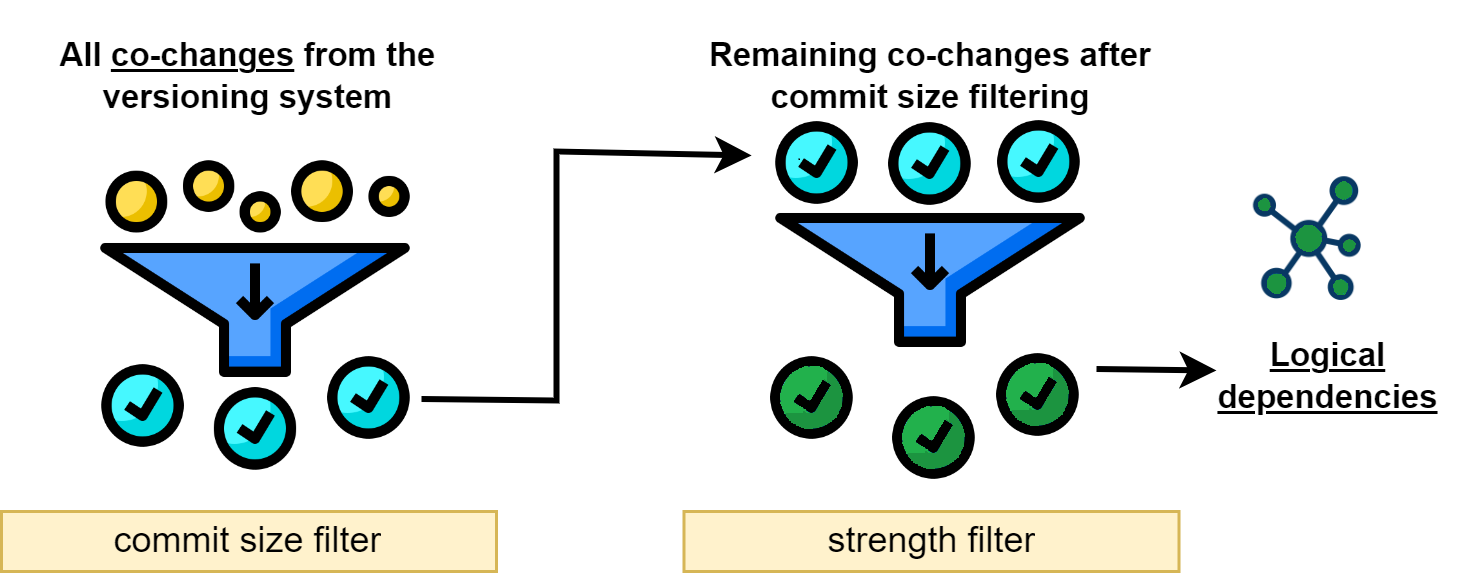
\includegraphics[width=\columnwidth]{filtering.png}
  \caption{ \textbf{Filter application process}}
  \label{fig:filtering}
\end{figure}

\subsubsection{Dependency Extraction and Filtering Tool}

We used a tool from our previous work \cite{b4} to extract co-changes from the versioning system and filter them into logical dependencies. This tool takes the GitHub repository address and the threshold values for commit and strength filters as input. The tool clones the repository, downloads all commit diffs starting from the first commit, examines all files changed in each commit to identify which entities have changed in those files, and creates undirected co-change dependencies between all changed entities within a commit.

The commit size filter is applied to these undirected co-change dependencies since the metric value for $(A \rightarrow B)$ is the same as for $(B \rightarrow A)$. For the strength filter, each co-change dependency is converted into a directed co-change dependency, so for each $(A \rightarrow B)$ dependency, we have both $(A \rightarrow B)$ and $(B \rightarrow A)$. This conversion is necessary because, as mentioned in the previous section, the confidence filter evaluates the rule's antecedent. Thus, the metric value for $(A \rightarrow B)$ differs from the metric value for $(B \rightarrow A)$.

After applying the filters, the remaining dependencies are exported for further use.

It is important to note that the strength metric is only used for filtering and is \textit{not considered as a weight} of the dependencies. \textit{The weight assigned to each dependency is the number of commits in which both entities were updated together}. This weight assignment reflects the frequency of co-change and indicates the strength of their logical connection. We chose this approach to maintain consistency with the weighting strategy used for structural dependencies, where more significant relationships are assigned higher weights. Based on the experiments presented in this paper, the average weights of logical dependencies are close in value to those of structural dependencies. This ensures that when the two types are combined, the weight distribution remains balanced and does not diminish the influence of structural dependencies in the dependency graph.


\subsubsection{Combining Structural and Logical Dependencies}

\Figure[t!](topskip=0pt, botskip=0pt, midskip=0pt)[width=\textwidth]{codegraph.png}
{ \textbf{Dependency Graph: Combining structural and logical dependencies.}\label{fig:codegraph}}

When structural dependencies (SD) and logical dependencies (LD) are combined in software clustering, both types of relationships are represented within the same graph.

Each entity in the system is represented as a node in the graph, and the dependencies between them are represented as directed weighted edges.

\textit{SD and LD weights are combined} when the same pair of entities appear in both dependencies. In this case, the weights from SD and LD are summed, giving more influence to those entity pairs. When a pair of entities appear only in SD or only in LD, the edge is added to the graph together with its corresponding weight. No normalization is applied during the combination; we rely on the SD predefined weights and the co-change frequency-derived LD weights to reflect the importance of each dependency type.

Figure \ref{fig:codegraph} illustrates combining structural and logical dependencies in the same dependency graph. The structural dependencies between \texttt{House}, \texttt{OrangeCat}, and \texttt{CatBehavior} entities are visible from the source code analysis.

However, the combination of SD and LD reveals additional insights. One important observation is the logical dependency between \texttt{House} and \texttt{OrangeCat}, which is not observed from the structural analysis. This relation is extracted from version control and filtered using a 60\% strength filter. The strength metric reveals that \texttt{House} and \texttt{OrangeCat} have a significant co-change value of 75.0, usually associated with a strong relationship.

When SD and LD overlap, such as between \texttt{OrangeCat} and \texttt{CatBehavior}, their weights are summed. This summation increases the weight of the dependency, making it more important in the dependency graph.



%%%%%%%%%%%%%%%%%%%%%%%%%%%%%%%%%%%%%%%%%%%%%%%%%%%%%


\section{Clustering Algorithms and Evaluation Metrics}
\label{sec:clustering_algorithms_evaluation}

In this section, we present the clustering algorithms used in our experiments: Louvain, Leiden, and DBSCAN. We also introduce the evaluation metrics used to assess the quality of the clustering results.


\subsection{Clustering Algorithms}

We selected Louvain, Leiden, and DBSCAN because they are scalable to systems of different sizes and compatible with the structure of our input data. Another important criterion was that the clustering algorithms should not require the number of clusters to be specified in advance. This is important in our context, where the number of expected modules is unknown. Louvain and Leiden are community detection algorithms designed for graph-based data, aligning with how we represent structural and logical dependencies. Leiden was included alongside Louvain because it addresses some of Louvain’s limitations.
DBSCAN was chosen because it offers a different clustering perspective. It can discover clusters of varying shapes and identify noise in the data. 

Using these three algorithms allows us to observe better how the type of input dependencies influences clustering results.

\subsubsection{Louvain}
\label{subsubsec:louvain}

The Louvain algorithm was originally developed by Blondel et al. and is used to find community partitions (clusters) in large networks. The algorithm begins with a weighted network of N nodes, initially assigning each node to its own cluster, resulting in N clusters. For each node, the algorithm evaluates the modularity gained from moving the node to the cluster of each of its neighbors. Based on the results, the node is moved to the cluster with the maximum positive modularity gain. This process is repeated for all nodes until no further improvement in modularity is possible \cite{b8}, \cite{b9}.

\subsubsection{Leiden}
\label{subsubsec:leiden}

The Leiden algorithm, developed by Traag et al., is an improvement over the Louvain algorithm for community detection in large networks. Like Louvain, the Leiden algorithm begins with each node assigned to its own cluster and iteratively moves nodes between clusters to optimize modularity. However, the Leiden algorithm addresses some problems of the Louvain method, particularly regarding poorly connected communities and runtime performance issues \cite{leiden} \cite{scikit}.

The Leiden algorithm introduces a refinement phase that ensures communities are locally optimally clustered and well-connected. This refinement step distinguishes the Leiden algorithm from Louvain.


\subsubsection{DBSCAN}
\label{subsubsec:dbscan}

The Density-Based Spatial Clustering of Applications with Noise (DBSCAN) algorithm, introduced by Ester et al., is a density-based clustering algorithm for identifying clusters of arbitrary shape and detecting noise in data \cite{dbscan}, \cite{scikit}.

DBSCAN operates based on two main parameters:

\begin{itemize}
\item \textbf{Eps}: It defines the radius within which to search for neighboring points.
\item \textbf{MinPts}: The minimum number of points required for a dense region. It determines the minimum number of neighbors a point should have to be considered a core point.
\end{itemize}

The algorithm classifies points into three categories:

\begin{enumerate}
\item \textbf{Core Points}: Points that have at least \textit{MinPts} neighbors within a radius of \textit{Eps}. These points are located in the interior of a cluster.
\item \textbf{Border Points}: Points that have fewer than \textit{MinPts} neighbors within a radius of \textit{Eps} but are in the Eps-neighborhood of a core point. They are located on the edge of a cluster.
\item \textbf{Noise}: Points that are neither core points nor border points.
\end{enumerate}

The DBSCAN algorithm starts by visiting an arbitrary point in the dataset. If the point is a core point, the algorithm starts a new cluster and retrieves all reachable points from this core point. All points are then marked as part of the cluster. If the point is a border point, it moves to the next point in the dataset. This process is repeated until all points have been visited.

DBSCAN can be applied for software clustering by considering software entities as data points. A distance measure based on dependency weights can be used to compute the neighborhood between entities.

\subsection{Clustering Result Evaluation}
\label{subsec:evaluation_def}

We evaluate the clustering results using two metrics: the Modularity Quality (MQ) metric and the Move and Join Effectiveness Measure (MoJoFM) metric. Each provides a different perspective on the quality of the clustering solutions. MQ reflects the internal structure and cohesiveness of the clusters, while MoJoFM offers an external perspective by comparing the result to a manually defined reference architecture.

\subsubsection{Modularity Quality Metric}
\label{subsec:mq}

Mancoridis et al. introduced the Modularity Quality (MQ) metric to evaluate the modularization quality of a clustering solution based on the interaction between modules (clusters) \cite{b101},\cite{b10}. It evaluates the difference between connections within clusters and connections between different clusters.

The MQ of a graph partitioned into \( k \) clusters, where \( A_i \) is the Intra-Connectivity of the \( i \)-th cluster and \( E_{ij} \) is the Inter-Connectivity between the \( i \)-th and \( j \)-th clusters, is calculated using Equation \eqref{eq:mq} \cite{b2}.

\begin{equation}
MQ = \left( \frac{1}{k} \sum_{i=1}^{k} A_i \right) - \left( \frac{1}{k(k-1)} \sum_{i,j=1}^{k} E_{ij} \right)
\label{eq:mq}
\end{equation}

The MQ metric's value ranges between -1 and 1. A value of -1 means that the clusters have more connections between the clusters than within the clusters, while a value of 1 means that there are more connections within clusters than between clusters. A good clustering solution should have an MQ value close to 1, since this indicates that the clusters are more cohesive internally and have fewer connections to other clusters. However, one limitation of MQ is that it can sometimes favor over-segmentation by rewarding small, tightly connected clusters. To address this, we also use the MoJoFM metric, defined in the next section, which helps identify such cases.

The MQ metric is useful because it does not require additional input besides the clustering result. It relies on the structure of the clustered entities and their interactions.

\subsubsection{MoJoFM Metric}
\label{subsec:mojofm}
Wen and Tzerpos introduced the MoJoFM metric to evaluate the similarity between two different software clustering results \cite{mojofm}. The metric is based on the MoJo metric, which measures the absolute minimum number of \textit{Move} and \textit{Join} operations required to transform one clustering solution into another \cite{b3}, \cite{mojofm}. However, MoJoFM provides a similarity measure ranging between 0\% and 100\%, where 100\% indicates identical clustering solutions.
Compared to the original MoJo metric, MoJoFM normalizes the result, making it easier to compare across different systems.

The MoJoFM metric is calculated using Equation \eqref{eq:mojofm}:

\begin{equation}
\text{MoJoFM}(A, B) = \left(1 - \frac{\text{mno}(A, B)}{\max(\text{mno}(\forall A, B))}\right) \times 100\%
\label{eq:mojofm}
\end{equation}

Where:

\begin{itemize}
\item $\text{mno}(A, B)$ is the minimum number of \textit{Move} and \textit{Join} operations required to transform clustering solution $A$ into clustering solution $B$.
\item $\max(\text{mno}(\forall A, B))$ is the maximum possible number of such operations required to transform any clustering $A$ into clustering $B$.
\end{itemize}

To use the metric, we first need to generate a reference clustering solution for comparison. We manually created this reference based on our analysis of the codebase, taking into account naming conventions, package structure, class responsibilities, and available documentation. While this reference is not considered an absolute ground truth, it is a practical baseline.

Using the MoJoFM metric, we can evaluate the similarity between the generated and reference clustering solutions. This metric is useful when combining multiple dependencies because it measures the similarity between the obtained clustering solutions and the same reference.

%%%%%%%%%%%%%%%%%%%%%%%%%%%%%%%%%%%%%%%%%%%%%%%%%%%%%%%%%%

\section{Tool Implementation and Workflow}
\label{sec:tool_workflow}

\Figure[t!](topskip=0pt, botskip=0pt, midskip=0pt)[width=\textwidth]{workflow-tool.png}
{ \textbf{Clustering tool workflow: input, graph construction, clustering, and evaluation.}\label{fig:tool}}

To evaluate how logical dependencies impact the quality of clustering solutions, we developed a Python tool capable of using any type of dependency, either alone or combined with other types of dependencies, as long as it is provided in CSV format. Structural dependencies are extracted from the source code using static analysis, and logical dependencies are extracted from version control history. Both types of dependencies are extracted using tools developed in our previous work. 

The tool clusters and evaluates software clustering solutions using the MQ or MoJoFM metrics.

The overall workflow of the tool, including the input, processing, and output steps described in more detail below, is shown in Figure \ref{fig:tool}.

\subsection{Input}

The tool takes one or multiple dependency CSV files as input and the reference solution required for the MoJoFM metric. We designed the tool to accept multiple dependency files so that we can generate clustering solutions based on either a single type of dependency (structural or logical) or a combination of both.

Since the MoJoFM metric requires a reference solution to evaluate the obtained clustering solutions, we manually inspected the code and created reference clustering solutions, which we then provided as input for the tool.

\subsection{Processing}

The dependencies are saved in the CSV file in the following format: \texttt{antecedent of a dependency, consequent of a dependency, weight}. The tool reads each line, adds the antecedent and consequent as nodes in a directed graph, and creates an edge between them, with the weight from the CSV file becoming the edge weight. The edge weights are summed if multiple dependency files are processed and the same dependency is found in multiple files. Self-loops cannot occur, as the input data consists only of pairs of distinct entities. Cycles are not explicitly handled or removed, as the clustering algorithms operate on the entire graph structure and are unaffected by their presence.

After all dependencies are read, the directed graph is passed to the clustering algorithms: Louvain, Leiden, and DBSCAN. For Louvain and Leiden, the clustering is applied directly to the directed graph. For DBSCAN, the graph is first converted into a symmetric distance matrix by combining the edge weights in both directions (e.g., from A to B and B to A), ensuring compatibility with the algorithm’s requirements. Each algorithm generates its own clustering result. The results from each algorithm are then evaluated using the MQ metric and the MoJoFM metric. The MQ metric requires the directed graph and the clustering result, while the MoJoFM metric requires the reference clustering solution provided as input and the clustering result.


\subsection{Output}

After applying each clustering algorithm and completing both evaluations, we export the clustering result, the number of clusters from the clustering solution, and the MQ and MoJoFM metrics values.


%%%%%%%%%%%%%%%%%%%%%%%%%%%%%%%%%%%%%%%%%%%%%%%%%%%%%%%%%%

\section{Experimental Plan}
\label{sec:plan}

This section presents the projects used in our experiments and the approach taken to conduct the experiments.

\subsection{Overview of projects used}
\begin{table*}
\centering
\caption{Overview of projects used in experimental analysis}
\label{tab:project_info}
\setlength{\tabcolsep}{7pt} 
\begin{tabular}{|l|l|c|l|p{4.7cm}|}
\hline
\textbf{Project Name} & \textbf{Release Tag} & \textbf{Commits} & \textbf{GitHub Repository Link} & \textbf{Repository Description} \\ 
 & \textbf{(Version)} & \textbf{Number} & &  \\ \hline
Apache Ant & \href{https://github.com/apache/ant/tree/rel/1.10.13}{rel/1.10.13} & 14917 & \href{https://github.com/apache/ant}{https://github.com/apache/ant} & Apache Ant is a Java-based build tool. \\ \hline
Apache Tomcat & \href{https://github.com/apache/tomcat/tree/8.5.93}{8.5.93} & 22698 & \href{https://github.com/apache/tomcat}{https://github.com/apache/tomcat} & 
Apache Tomcat is an open-source Java web server and servlet container\\ \hline
Hibernate ORM & \href{https://github.com/hibernate/hibernate-orm/tree/6.2.14}{6.2.14} & 16609 & \href{https://github.com/hibernate/hibernate-orm}{https://github.com/hibernate/hibernate-orm} & Hibernate ORM is a Java-based object-relational mapping (ORM) framework for managing database interactions. \\ \hline
Gson & \href{https://github.com/google/gson/tree/gson-parent-2.10.1}{gson-parent-2.10.1} & 1772 & \href{https://github.com/google/gson}{https://github.com/google/gson} & A Java library for transforming Java objects into JSON format and reconstructing them back. \\ \hline
\end{tabular}
\end{table*}

In Table \ref{tab:project_info}, we have synthesized all the information about the four projects used in our experiments. The 'Project Name' column contains the names of the software projects sourced from GitHub. The 'Release Tag' column contains the specific release tag of the project that was analyzed. We processed all the commits for logical dependency extraction, from the first commit to the commit associated with the specified tag. We extracted the dependencies from the code of that specific tag for structural dependencies. The 'Number of Commits' column provides the total number of commits used for logical dependencies extraction. The 'GitHub Repository Link' column includes the URL link to the project's repository on GitHub. Finally, the 'Repository Description' column briefly describes the project's purpose and functionality.

We mainly chose projects with more than 10,000 commits in their commit history so that the logical dependencies extraction can be done on a more extensive information base. However, we selected Gson, which has a relatively small commit history (1,772 commits), to determine if our experiments work with a smaller information base.

\subsection{Tool runs}

To assess the impact of logical dependencies and to answer the research questions from section \ref{sec:introduction}, we run the tool presented in Section \ref{sec:tool_workflow} in three different scenarios for all the projects from table \ref{tab:project_info}. All three scenarios are illustrated in Fig. \ref{fig:scenatrio}.

In the first scenario, we run the tool once, providing only the system's structural dependencies as input for the clustering algorithm.

In the second scenario, we run the tool ten times, using only logical dependencies as input. Each run corresponds to a different strength threshold value applied when filtering co-changes during logical dependency extraction. We generate a new logical dependency file for each threshold value, starting with a threshold of 10 and increasing in increments of 10, up to and including 100. A threshold of 0 is not used since a strength value of 0\% is not possible by the definition of the strength metric. There must be at least one co-change event between two entities to compute a valid strength value. We start at 10\% as a practical lower bound to avoid including a large number of low-confidence, noisy dependencies. The maximum threshold is set to 100\%, as strength metric values are clipped to a maximum of 100.
This results in ten separate CSV files, each containing a different subset of logical dependencies, which are then used as input for clustering.

In the third scenario, we combine logical with structural dependencies. Similar to the second scenario, we ran the tool ten times using structural and logical dependencies generated with different strength thresholds.

\begin{figure}[t!]
  \centering
  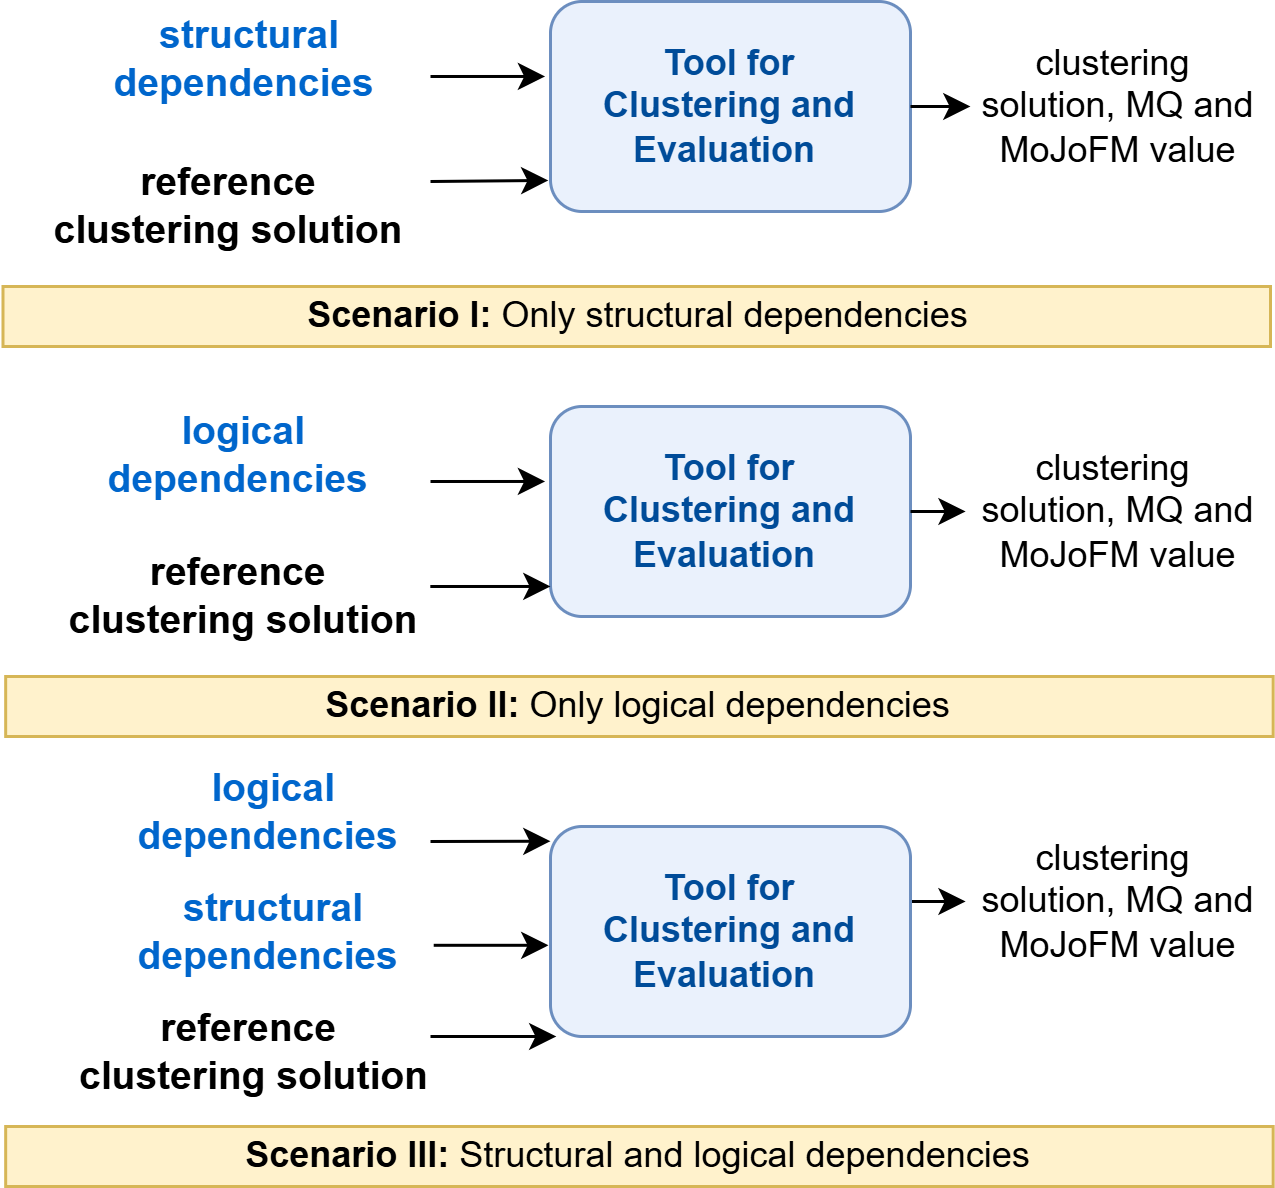
\includegraphics[width=\columnwidth]{scenario.png}
  \caption{ \textbf{Experimental scenarios for analyzing the impact of logical dependencies on clustering quality}}
  \label{fig:scenatrio}
\end{figure}


\subsection{Computing Environment}

All experiments were conducted on a local machine with an Intel(R) Core(TM) i7-8665U CPU, using Windows 10. The implementation was done in Python 3.10.


\section{Experimental Results}
\label{sec:results}

The experimental results are presented in this section in four tables, each corresponding to a different project. Table \ref{tab:clustering_results_ant} presents the results for Apache Ant, Table \ref{tab:clustering_results_tomcat} presents the results for Apache Tomcat, Table \ref{tab:clustering_results_hibernate} presents the results for Hibernate ORM, and Table \ref{tab:clustering_results_gson} presents the results for Gson.

Each table includes the following columns:
\begin{itemize}
\item \textbf{Dependency Type:} The types of dependencies used are as follows: SD for Structural Dependencies, LD for Logical Dependencies, and SD+LD for their combination. The strength threshold used is specified in parentheses right after LD.
\item \textbf{Entities Count:} The total number of software entities (such as classes, interfaces, enums) involved in clustering.
\item \textbf{System Coverage:} Considering that the total number of entities extracted from the codebase — which represents the entities forming structural dependencies (SD) — constitutes the entire set of entities in the system (the first line of each table), we calculated the percentage of entities present in the filtered logical dependencies (LD) relative to the total number of known codebase entities.
\item \textbf{Louvain/ Leiden/ DBSCAN:} The clustering algorithms used in the experiments.
\item \textbf{Nr. of Clusters:} The number of clusters from the clustering solution.
\item \textbf{MQ (Modularization Quality):} The result obtained when applying the MQ evaluation metric to the clustering solution.
\item \textbf{MoJoFM:} The result obtained when applying the MoJoFM evaluation metric to the clustering solution.
\end{itemize}

The rows in each table represent different dependency types and strength filter thresholds used in the clustering experiments.



\begin{table*}[htbp]
\centering
\caption{Clustering results based on different dependency types and strength filter thresholds for repository: \url{https://github.com/apache/ant}}
\label{tab:clustering_results_ant}
\setlength{\tabcolsep}{7pt} 
\begin{tabular}{|l|c|c|ccc|ccc|ccc|}
\hline
 \textbf{Dependency} &  \textbf{Entities} & \textbf{System} & \multicolumn{3}{c|}{\textbf{Louvain}} & \multicolumn{3}{c|}{\textbf{Leiden}} & \multicolumn{3}{c|}{\textbf{DBSCAN}} \\
\cline{4-12}
\textbf{Type (strength } &  \textbf{Count} & \textbf{Coverage} & \textbf{Nr. of } & \textbf{MQ} & \textbf{MojoFM} & \textbf{Nr. of} & \textbf{MQ} & \textbf{MojoFM} & \textbf{Nr. of} & \textbf{MQ} & \textbf{MojoFM}  \\
\textbf{threshold)} &  & \textbf{(\%)} & \textbf{clusters} & & & \textbf{clusters} & &  & \textbf{clusters} & &\\
\hline
\rowcolor[HTML]{ECECEC} \textbf{SD} & 517 & 100.00 & 14 & 0.114 & 46.02 & 14 & 0.101 & 52.99 & 34 & 0.144 & 25.1  \\
\textbf{LD (10)} & 320 & 61.89 & 55 & 0.506 & 65.57 & 55 & 0.506 & 65.57 & 30 & 0.435 & 39.02 \\
\textbf{LD (20)} & 215 & 41.58 & 53 & 0.547 & 68 & 53 & 0.547 & 68 & 23 & 0.505 & 53.5 \\
\textbf{LD (30)} & 174 & 33.65 & 44 & 0.558 & 71.7 & 44 & 0.558 & 71.7 & 19 & 0.585 & 50 \\
\textbf{LD (40)} & 152 & 29.40 & 40 & 0.580 & 71.53 & 40 & 0.580 & 71.53 & 19 & 0.602 & 53.06 \\
\textbf{LD (50)} & 138 & 26.69 & 35 & 0.604 & 73.98 & 35 & 0.604 & 73.98 & 17 & 0.633 & 56.1 \\
\textbf{LD (60)} & 120 & 23.21 & 34 & 0.587 & 70.48 & 34 & 0.587 & 70.48 & 14 & 0.650 & 51.43 \\
\textbf{LD (70)} & 106 & 20.50 & 32 & 0.577 & 71.43 & 32 & 0.577 & 71.43 & 11 & 0.661 & 51.65 \\
\textbf{LD (80)} & 92 & 17.79 & 29 & 0.576 & 70.13 & 29 & 0.576 & 70.13 & 9 & \cellcolor[HTML]{FEF9E4}0.709 & 50.65 \\
\textbf{LD (90)} & 79 & 15.28 & 24 & 0.606 & 71.88 & 24 & 0.606 & 71.88 & 8 & 0.705 & 56.6 \\
\textbf{LD (100)} & 64 & 12.37 & 19 & \cellcolor[HTML]{fef9e4}0.611 & \cellcolor[HTML]{fef9e4}75.51 & 19 & \cellcolor[HTML]{fef9e4}0.611 & \cellcolor[HTML]{fef9e4}75.51 & 6 & 0.691 & \cellcolor[HTML]{fef9e4}56.93 \\
\hline
\textbf{SD+LD (10)} & 517 & 100.00 & 18 & \cellcolor[HTML]{fef9e4}0.355 & \cellcolor[HTML]{fef9e4}55.18 & 15 & 0.254 & \cellcolor[HTML]{fef9e4}54.98 & 37 & 0.147 & 25.9 \\
\textbf{SD+LD (20)} & 517 & 100.00 & 17 & 0.318 & 52.39 & 19 & \cellcolor[HTML]{fef9e4}0.365 & 53.78 & 32 & 0.149 & \cellcolor[HTML]{fef9e4}26.49 \\
\textbf{SD+LD (30)} & 517 & 100.00 & 16 & 0.282 & 53.19 & 16 & 0.265 & 54.78 & 30 & \cellcolor[HTML]{FEF9E4}0.159 & 24.5 \\
\textbf{SD+LD (40)} & 517 & 100.00 & 17 & 0.340 & 51.99 & 17 & 0.317 & 53.19 & 31 & 0.146 & 24.7 \\
\textbf{SD+LD (50)} & 517 & 100.00 & 15 & 0.248 & 52.59 & 19 & 0.298 & 56.77 & 31 & 0.146 & 24.7 \\
\textbf{SD+LD (60)} & 517 & 100.00 & 16 & 0.244 & 50.8 & 16 & 0.271 & 54.38 & 32 & 0.155 & 25.1 \\
\textbf{SD+LD (70)} & 517 & 100.00 & 15 & 0.238 & 51.00 & 18 & 0.281 & 52.99 & 32 & 0.155 & 25.1 \\
\textbf{SD+LD (80)} & 517 & 100.00 & 13 & 0.246 & 45.22 & 15 & 0.255 & 45.82 & 32 & 0.155 & 25.1 \\
\textbf{SD+LD (90)} & 517 & 100.00 & 14 & 0.258 & 46.02 & 16 & 0.268 & 47.01 & 32 & 0.155 & 25.1 \\
\textbf{SD+LD (100)} & 517 & 100.00 & 15 & 0.214 & 50.8 & 15 & 0.227 & 50.4 & 32 & 0.155 & 25.1 \\
\hline
\end{tabular}
\end{table*}



\begin{table*}[htbp]
\centering
\caption{Clustering results based on different dependency types and strength filter thresholds for repository: \href{https://github.com/apache/tomcat}{https://github.com/apache/tomcat}}
\label{tab:clustering_results_tomcat}
\setlength{\tabcolsep}{7pt} 
\begin{tabular}{|l|c|c|ccc|ccc|ccc|}
\hline
 \textbf{Dependency} &  \textbf{Entities} & \textbf{System} & \multicolumn{3}{c|}{\textbf{Louvain}} & \multicolumn{3}{c|}{\textbf{Leiden}} & \multicolumn{3}{c|}{\textbf{DBSCAN}} \\
\cline{4-12}
\textbf{Type (strength } &  \textbf{Count} & \textbf{Coverage} & \textbf{Nr. of } & \textbf{MQ} & \textbf{MojoFM} & \textbf{Nr. of} & \textbf{MQ} & \textbf{MojoFM} & \textbf{Nr. of} & \textbf{MQ} & \textbf{MojoFM}  \\
\textbf{threshold)} &  & \textbf{(\%)} & \textbf{clusters} & & & \textbf{clusters} & &  & \textbf{clusters} & &\\
\hline
\rowcolor[HTML]{ECECEC} \textbf{SD} & 662 & 100.00 & 26 & 0.186 & 77.76 & 24 & 0.184 & 76.99 & 43 & 0.142 & 73.31  \\
\textbf{LD (10)} & 406 & 61.33 & 42 & 0.505 & 72.47 & 42 & 0.505 & 72.47 & 60 & 0.393 & 67.93 \\
\textbf{LD (20)} & 303 & 45.77 & 45 & 0.538 & 68.26 & 45 & 0.538 & 67.24 & 41 & 0.510 & 72.7 \\
\textbf{LD (30)} & 249 & 37.61 & 46 & 0.532 & 69.87 & 46 & 0.532 & 69.87 & 32 & 0.561 & 80.33 \\
\textbf{LD (40)} & 208 & 31.42 & 42 & 0.590 & 69.70 & 42 & 0.591 & 70.71 & 28 & 0.572 & 83.84 \\
\textbf{LD (50)} & 198 & 29.91 & 44 & 0.604 & 70.21 & 44 & 0.604 & 70.21 & 22 & 0.631 & 85.11 \\
\textbf{LD (60)} & 177 & 26.74 & 45 & 0.601 & 70.66 & 45 & 0.601 & 70.66 & 18 & 0.662 & 85.63 \\
\textbf{LD (70)} & 164 & 24.77 & 45 & 0.598 & 75.32 & 45 & 0.598 & 75.32 & 17 & 0.676 & 88.96 \\
\textbf{LD (80)} & 127 & 19.18 & 36 & 0.618 & 79.49 & 36 & 0.618 & 79.49 & 15 & 0.713 & \cellcolor[HTML]{fef9e4}89.74 \\
\textbf{LD (90)} & 116 & 17.52 & 32 & 0.623 & 81.13 & 32 & 0.623 & 81.13 & 14 & 0.718 & 89.62 \\
\textbf{LD (100)} & 110 & 16.62 & 30 & \cellcolor[HTML]{fef9e4}0.640 & \cellcolor[HTML]{fef9e4}85.00 & 30 & \cellcolor[HTML]{fef9e4}0.640 & \cellcolor[HTML]{fef9e4}85.00 & 13 & \cellcolor[HTML]{fef9e4}0.735 & 89.00 \\
\hline
\textbf{SD+LD(10)} & 662 & 100.00 & 28 & \cellcolor[HTML]{fef9e4}0.324 & 78.99 & 28 & 0.324 & 78.99 & 40 & 0.161 & \cellcolor[HTML]{fef9e4}74.23 \\
\textbf{SD+LD(20)} & 662 & 100.00 & 31 & 0.287 & 78.22 & 30 & 0.320 & \cellcolor[HTML]{fef9e4}80.06 & 50 & 0.189 & 73.31 \\
\textbf{SD+LD(30)} & 662 & 100.00 & 32 & 0.296 & \cellcolor[HTML]{fef9e4}79.92 & 32 & 0.277 & 75.77 & 45 & \cellcolor[HTML]{fef9e4}0.209 & 73.47 \\
\textbf{SD+LD(40)} & 662 & 100.00 & 34 & 0.292 & 79.91 & 32 & \cellcolor[HTML]{fef9e4}0.326 & 78.22 & 43 & 0.198 & 73.47 \\
\textbf{SD+LD(50)} & 662 & 100.00 & 33 & 0.294 & 76.53 & 35 & 0.301 & 76.23 & 43 & 0.196 & 73.31 \\
\textbf{SD+LD(60)} & 662 & 100.00 & 35 & 0.304 & 77.15 & 33 & 0.286 & 76.84 & 41 & 0.177 & 73.62 \\
\textbf{SD+LD(70)} & 662 & 100.00 & 34 & 0.282 & 76.69 & 34 & 0.292 & 77.45 & 41 & 0.166 & 73.62 \\
\textbf{SD+LD(80)} & 662 & 100.00 & 34 & 0.283 & 76.23 & 33 & 0.282 & 76.38 & 42 & 0.153 & 73.47 \\
\textbf{SD+LD(90)} & 662 & 100.00 & 31 & 0.311 & 78.99 & 31 & 0.311 & 78.99 & 43 & 0.153 & 73.31 \\
\textbf{SD+LD(100)} & 662 & 100.00 & 31 & 0.311 & 78.83 & 31 & 0.305 & 78.37 & 43 & 0.153 & 73.31 \\
\hline
\end{tabular}
\end{table*}




\begin{table*}[htbp]
\centering
\caption{Clustering results based on different dependency types and strength filter thresholds for repository: \href{https://github.com/hibernate/hibernate-orm}{https://github.com/hibernate/hibernate-orm}}
\label{tab:clustering_results_hibernate}
\setlength{\tabcolsep}{7pt} 
\begin{tabular}{|l|c|c|ccc|ccc|ccc|}
\hline
 \textbf{Dependency} &  \textbf{Entities} & \textbf{System} & \multicolumn{3}{c|}{\textbf{Louvain}} & \multicolumn{3}{c|}{\textbf{Leiden}} & \multicolumn{3}{c|}{\textbf{DBSCAN}} \\
\cline{4-12}
\textbf{Type (strength } &  \textbf{Count} & \textbf{Coverage} & \textbf{Nr. of } & \textbf{MQ} & \textbf{MojoFM} & \textbf{Nr. of} & \textbf{MQ} & \textbf{MojoFM} & \textbf{Nr. of} & \textbf{MQ} & \textbf{MojoFM}  \\
\textbf{threshold)} &  & \textbf{(\%)} & \textbf{clusters} & & & \textbf{clusters} & &  & \textbf{clusters} & &\\
\hline
\rowcolor[HTML]{ECECEC} \textbf{SD} & 4414 & 100.00 & 30 & 0.09 & 52.23 & 23 & 0.071 & 52.44 & 373 & 0.128 & 46.32  \\
\textbf{LD (10)} & 1450 & 32.85 & 44 & 0.389 & 57.22 & 45 & 0.39 & 58.22 & 99 & 0.395 & 57.08 \\
\textbf{LD (20)} & 1325 & 30.02 & 66 & 0.397 & 62.66 & 66 & 0.397 & 62.66 & 151 & 0.378 & 63.36 \\
\textbf{LD (30)} & 1222 & 27.68 & 66 & 0.38 & 62.45 & 67 & 0.38 & 63.04 & 148 & 0.378 & 65.42 \\
\textbf{LD (40)} & 915 & 20.73 & 84 & 0.417 & 63.68 & 85 & 0.412 & 63.56 & 110 & 0.382 & 66.9 \\
\textbf{LD (50)} & 900 & 20.39 & 84 & 0.409 & 64.56 & 84 & 0.409 & 64.56 & 105 & 0.386 & 67.02 \\
\textbf{LD (60)} & 848 & 19.21 & 82 & 0.406 & 63.26 & 81 & 0.41 & 63.39 & 104 & 0.379 & 65.13 \\
\textbf{LD (70)} & 459 & 10.40 & 89 & 0.516 & \cellcolor[HTML]{fef9e4}69.08 & 89 & 0.516 & \cellcolor[HTML]{fef9e4}69.08 & 41 & 0.467 & 58.21 \\
\textbf{LD (80)} & 450 & 10.19 & 91 & 0.506 & 68.64 & 91 & 0.506 & 68.64 & 39 & 0.479 & \cellcolor[HTML]{fef9e4}60.49 \\
\textbf{LD (90)} & 432 & 9.79 & 92 & 0.492 & 66.93 & 92 & 0.492 & 66.93 & 40 & 0.473 & 58.66 \\
\textbf{LD (100)} & 356 & 8.07 & 81 & \cellcolor[HTML]{fef9e4}0.524 & 65.92 & 81 & \cellcolor[HTML]{fef9e4}0.524 & 65.92 & 29 & \cellcolor[HTML]{fef9e4}0.537 & 58.2 \\
\hline
\textbf{SD+LD (10)} & 4414 & 100.00 & 19 & 0.096 & 53.93 & 19 & 0.099 & 52.28 & 282 & 0.121 & 46.01 \\
\textbf{SD+LD (20)} & 4414 & 100.00 & 21 & 0.126 & 52.85 & 23 & 0.122 & 56.21 & 309 & \cellcolor[HTML]{fef9e4}0.135 & 47.4 \\
\textbf{SD+LD (30)} & 4414 & 100.00 & 26 & 0.121 & 55.76 & 26 & 0.15 & 54.54 & 317 & 0.135 & \cellcolor[HTML]{fef9e4}49.45 \\
\textbf{SD+LD (40)} & 4414 & 100.00 & 27 & \cellcolor[HTML]{fef9e4}0.182 & \cellcolor[HTML]{fef9e4}54.57 & 28 & \cellcolor[HTML]{fef9e4}0.163 & \cellcolor[HTML]{fef9e4}55.89 & 350 & 0.134 & 49.35 \\
\textbf{SD+LD (50)} & 4414 & 100.00 & 26 & 0.16 & 52.37 & 24 & 0.147 & 53.31 & 350 & 0.134 & 49.37 \\
\textbf{SD+LD (60)} & 4414 & 100.00 & 26 & 0.161 & 52.35 & 27 & 0.153 & 53.19 & 352 & 0.135 & 49.31 \\
\textbf{SD+LD (70)} & 4414 & 100.00 & 28 & 0.139 & 52.78 & 29 & 0.154 & 54.34 & 366 & 0.13 & 47.13 \\
\textbf{SD+LD (80)} & 4414 & 100.00 & 28 & 0.142 & 52.83 & 28 & 0.147 & 53.35 & 366 & 0.13 & 47.72 \\
\textbf{SD+LD (90)} & 4414 & 100.00 & 28 & 0.136 & 52.62 & 30 & 0.153 & 53.83 & 365 & 0.13 & 47.72 \\
\textbf{SD+LD (100)} & 4414 & 100.00 & 30 & 0.128 & 52.78 & 28 & 0.114 & 55.23 & 365 & 0.128 & 47.75 \\
\hline
\end{tabular}
\end{table*}






\begin{table*}[htbp]
\centering
\caption{Clustering results based on different dependency types and strength filter thresholds for repository: \href{https://github.com/google/gson}{https://github.com/google/gson}}
\label{tab:clustering_results_gson}
\setlength{\tabcolsep}{7pt} 
\begin{tabular}{|l|c|c|ccc|ccc|ccc|}
\hline
 \textbf{Dependency} &  \textbf{Entities} & \textbf{System} & \multicolumn{3}{c|}{\textbf{Louvain}} & \multicolumn{3}{c|}{\textbf{Leiden}} & \multicolumn{3}{c|}{\textbf{DBSCAN}} \\
\cline{4-12}
\textbf{Type (strength } &  \textbf{Count} & \textbf{Cover} & \textbf{Nr. of } & \textbf{MQ} & \textbf{MojoFM} & \textbf{Nr. of} & \textbf{MQ} & \textbf{MojoFM} & \textbf{Nr. of} & \textbf{MQ} & \textbf{MojoFM}  \\
\textbf{threshold)} &  & \textbf{(\%)} & \textbf{clusters} & & & \textbf{clusters} & &  & \textbf{clusters} & &\\
\hline
\rowcolor[HTML]{ECECEC} \textbf{gson SD} & 210 & 100.00 & 10 & 0.139 & 53.47 & 9 & 0.129 & 55.94 & 23 & 0.127 & 51.88 \\
\textbf{gson LD (10)} & 66 & 31.43 & 10 & 0.565 & 62.07 & 9 & 0.572 & 60.34 & 19 & 0.399 & 68.97 \\
\textbf{gson LD (20)} & 50 & 23.81 & 11 & 0.547 & 64.29 & 11 & 0.547 & 64.29 & 9 & 0.523 & 59.52 \\
\textbf{gson LD (30)} & 41 & 19.52 & 12 & 0.544 & 63.64 & 12 & 0.544 & 63.64 & 6 & 0.606 & 66.67 \\
\textbf{gson LD (40)} & 31 & 14.76 & 8 & \cellcolor[HTML]{fef9e4}0.635 & \cellcolor[HTML]{fef9e4}69.57 & 8 & \cellcolor[HTML]{fef9e4}0.635 & \cellcolor[HTML]{fef9e4}69.57 & 6 & \cellcolor[HTML]{fef9e4}0.612 & \cellcolor[HTML]{fef9e4}69.57 \\
\textbf{gson LD (50)} & 31 & 14.76 & 8 & 0.600 & 69.57 & 8 & 0.600 & 69.57 & 6 & 0.565 & 60.87 \\
\textbf{gson LD (60)} & 28 & 13.33 & 8 & 0.552 & 65.00 & 8 & 0.552 & 65.00 & 5 & 0.584 & 60.00 \\
\textbf{gson LD (70)} & 26 & 12.38 & 7 & 0.579 & 66.67 & 7 & 0.579 & 66.67 & 5 & 0.586 & 55.56 \\
\textbf{gson LD (80)} & 18 & 8.57 & 5 & 0.590 & 60.00 & 5 & 0.590 & 60.00 & 4 & 0.544 & 40.00 \\
\textbf{gson LD (90)} & 18 & 8.57 & 5 & 0.590 & 60.00 & 5 & 0.590 & 60.00 & 4 & 0.544 & 40.00 \\
\textbf{gson LD (100)} & 18 & 8.57 & 5 & 0.590 & 60.00 & 5 & 0.590 & 60.00 & 4 & 0.544 & 40.00 \\
\hline
\textbf{gson SD+LD(10)} & 210 & 100.00 & 11 & \cellcolor[HTML]{fef9e4}0.317 & \cellcolor[HTML]{fef9e4}64.36 & 11 & \cellcolor[HTML]{fef9e4}0.317 & \cellcolor[HTML]{fef9e4}64.36 & 20 & \cellcolor[HTML]{fef9e4}0.172 & \cellcolor[HTML]{fef9e4}63.86 \\
\textbf{gson SD+LD(20)} & 210 & 100.00 & 11 & 0.259 & 61.39 & 11 & 0.259 & 61.39 & 17 & 0.136 & 53.96 \\
\textbf{gson SD+LD(30)} & 210 & 100.00 & 11 & 0.277 & 61.39 & 11 & 0.277 & 61.39 & 20 & 0.136 & 55.94 \\
\textbf{gson SD+LD(40)} & 210 & 100.00 & 10 & 0.277 & 61.39 & 10 & 0.277 & 61.39 & 20 & 0.135 & 55.94 \\
\textbf{gson SD+LD(50)} & 210 & 100.00 & 10 & 0.270 & 60.40 & 11 & 0.270 & 60.89 & 20 & 0.135 & 55.94 \\
\textbf{gson SD+LD(60)} & 210 & 100.00 & 9 & 0.296 & 61.39 & 10 & 0.290 & 61.88 & 20 & 0.135 & 55.94 \\
\textbf{gson SD+LD(70)} & 210 & 100.00 & 8 & 0.295 & 59.41 & 8 & 0.295 & 59.41 & 20 & 0.135 & 55.94 \\
\textbf{gson SD+LD(80)} & 210 & 100.00 & 7 & 0.267 & 58.91 & 8 & 0.263 & 59.41 & 21 & 0.134 & 55.45 \\
\textbf{gson SD+LD(90)} & 210 & 100.00 & 7 & 0.267 & 58.91 & 7 & 0.267 & 58.91 & 21 & 0.134 & 55.45 \\
\textbf{gson SD+LD(100)} & 210 & 100.00 & 7 & 0.267 & 58.91 & 8 & 0.263 & 59.41 & 21 & 0.134 & 55.45 \\
\hline
\end{tabular}
\end{table*}


\begin{table}[htbp]
\centering
\begin{tabular}{|c|c|c|c|c|}
\hline
\textbf{Dependency type} & \textbf{Ant} & \textbf{Tomcat} & \textbf{Hibernate} & \textbf{Gson} \\ \hline
\rowcolor[HTML]{ECECEC}\textbf{SD}     & 5.91  & 6.91  & 5.41  & 5.24  \\
\textbf{LD(10)} & 11.17 & 12.82 & 2.45  & 14.15 \\
\textbf{LD(20)} & 16.01 & 19.65 & 3.00  & 19.10 \\ 
\textbf{LD(30)} & 18.08 & 23.56 & 3.27  & 27.58 \\ 
\textbf{LD(40)} & 19.08 & 25.57 & 4.63  & 29.85 \\ 
\textbf{LD(50)} & 19.94 & 26.31 & 4.80  & 29.97 \\ 
\textbf{LD(60)} & 24.26 & 28.91 & 5.14  & 33.93 \\ 
\textbf{LD(70)} & 26.70 & 30.35 & 9.53  & 34.37 \\ 
\textbf{LD(80)} & 30.83 & 35.33 & 10.18 & 43.00 \\ 
\textbf{LD(90)} & 32.11 & 36.90 & 10.47 & 43.00 \\ 
\textbf{LD(100)} & 33.93 & 37.04 & 12.00 & 43.00 \\
 \hline
\end{tabular}
\caption{Average weights of Structural Dependencies (SD) and Logical Dependencies (LD).}
\label{tab:systems_weights}
\end{table}


To better understand the impact of different dependency types on software clustering, we also analyzed the average weights assigned to structural dependencies (SD) and logical dependencies (LD) across the studied projects. Table \ref{tab:systems_weights} presents these average dependency weights. The first row shows the average weights for SD, which remain constant across all strength thresholds, while the other rows show the average weights for logical dependencies at different strength thresholds.


The overall analysis of all the results from this section indicates that combining structural and logical dependencies (SD+LD) provides better clustering solutions than using structural dependencies (SD) alone, covering 100\% of the system, meaning that no entity is missed during cluster generation. On the other hand, logical dependencies (LD) alone result in better clustering quality metrics compared to both SD and SD+LD, but they do not cover the entire system.

The best results for SD+LD are observed with a strength threshold between 10-40\%. For LD only, the best results are obtained at a 100\% strength threshold. The overall trend shows that for LD only, the MQ metric increases in value with a higher strength threshold, indicating more cohesive clusters, while the MoJo metric decreases, indicating that fewer transformations are needed to reach the expected clustering. For SD+LD, the best MQ and MoJo values are obtained at lower strength thresholds, and then both metrics indicate a less effective clustering solution obtained with higher strength thresholds.

We analyze each project in detail in the sections below.

\subsection{Apache Ant}

The clustering results for Apache Ant (Table \ref{tab:clustering_results_ant}) show that the combined structural and logical dependencies (SD+LD) achieved the best values with a strength threshold between 10\% and 30\%. The highest value for the MQ metric is reached with Leiden at a strength threshold of 20\%, and the highest value for MoJoFM is also reached with Leiden at a strength threshold of 10\%.

Compared with the SD-only results, all SD+LD clustering solutions for all algorithms show better MQ metric values, with the highest MQ value for SD+LD being more than three times greater than the corresponding SD-only value. Similarly, the MoJoFM metric shows better results than SD-only. However, it does not always outperform the MoJoFM metric applied to SD-only data.

Logical dependencies (LD) alone produced the highest MQ and MoJoFM values at the 100\% strength threshold for both Leiden and Louvain, with the obtained metric values being higher than those of SD-only and SD+LD. However, the percentage of entities covered is significantly lower (LD(100) covers only 12.37\% of the system).
If we look at LD(10), where there is a 61.89\% coverage of the system, which is more compared to LD(100), both metrics still perform better than SD-only and SD+LD(10). However, there is still a gap until 100\% coverage.

From the clustering algorithm performance point of view, Leiden obtains the best evaluation metrics for all scenarios, followed by Louvain and DBSCAN.

One interesting observation is that, based on the LD-only results, where the metrics results improved with higher strength thresholds, the SD+LD results did not follow the same pattern. On the opposite, the SD+LD metric results decline with a higher strength threshold. An explanation for this behavior may lie in the overlap between structural and logical dependencies. As presented in Figure \ref{fig:ant_correlation}, the number of LD decreases with a stricter strength threshold compared to the number of SD, and the overlap between the two types of dependencies increases.

\begin{figure}[t!]
\centering
\includegraphics[width=\columnwidth]{ant_correlation.png}
\caption{\textbf{Apache Ant: Overlap between structural and logical dependencies and its correlation with clustering metrics.}}
\label{fig:ant_correlation}
\end{figure}

In our previous works, we studied how these two types of dependencies overlap \cite{b4}, \cite{b5}. The reason behind those studies was to check how much new information we can get from using logical dependencies and how much is already present via structural dependencies.

Our overall findings were that with stricter filtering of logical dependencies, we obtain a higher percentage of overlap between the two dependencies, reaching at most 50\% of logical dependencies that are also structural dependencies.

So, we consider that the reason why SD+LD clustering solutions decline in performance with a higher strength threshold is that less and less new additional information is added to the system (logical dependencies that are not structural dependencies), causing the clustering solution to start resembling the performance of the SD-only solution. In Figure \ref{fig:ant_correlation}, we can see that LD(10) represents 61\% of the quantity of SD, while LD(100) is only at 12\%, with half of them being duplicated with SD.

\subsection{Apache Tomcat}

For Apache Tomcat (Table \ref{tab:clustering_results_tomcat}), the best results for SD+LD were obtained with strength thresholds between 10\% and 40\% across all algorithms. The Leiden algorithm achieved the best result for the MQ metric at a strength threshold of 40\%, while the best MoJoFM result was obtained at a threshold of 20\%, also with the Leiden algorithm. Compared with the SD-only results, the peak MQ values almost double the SD-only values. Like Apache Ant, the MQ values for all strength thresholds are higher than those for SD-only. While MoJoFM is not better for all thresholds, it still improves compared with the SD-only results.

The LD-only results show the highest MQ and MoJoFM values at LD(100) for the Louvain and Leiden algorithms. However, as with the Apache Ant results, coverage remains an issue. LD(100) covers only 16.62\% of the system, lower than the coverage from SD-only or SD+LD combinations. On the other hand, LD(10), which covers 61.33\% of the system, still has better clustering solutions compared to SD-only, based on both MQ and MoJoFM results.

We observe the same decline in results with a stricter strength threshold for SD+LD. As with the previous system, these results can again be connected to the percentage of LD that also overlaps with SD and the decreasing number of LD compared to SD once the strength threshold becomes stricter. As shown in Figure \ref{fig:catalina_correlation}, LD filtered with a 10\% strength threshold overlaps with SD by approximately 22\%, while at a 100\% strength threshold, the overlap increases to approximately 39\%.

\begin{figure}[t!]
\centering
\includegraphics[width=\columnwidth]{catalina_correlation.png}
\caption{\textbf{Apache Tomcat: Overlap between structural and logical dependencies and its correlation with clustering metrics.}}
\label{fig:catalina_correlation}
\end{figure}

To ensure that the decline in performance for SD+LD with a stricter strength threshold is indeed caused by the fact that LD are significantly fewer than SD, and SD duplicates that part of them at higher thresholds, we added an additional experiment to our study. In this experiment, whose results can be found in Table \ref{tab:clustering_results_multiplication}, we increased the weights associated with LD(100) for Apache Tomcat to confirm that we are dealing with an LD quantity problem rather than a weight problem.

Therefore, in this experiment, we increased the weight assigned to each logical dependency filtered with a 100\% strength threshold from the Apache Tomcat system by values ranging from 1 to 5 and re-ran scenario III from Fig. \ref{fig:scenatrio}.


To maintain consistency, we used the same columns as in the other result tables (\ref{tab:clustering_results_ant}, \ref{tab:clustering_results_tomcat}, \ref{tab:clustering_results_hibernate}, \ref{tab:clustering_results_gson}), with the addition of two new columns:
\begin{itemize}
\item \textbf{Multiplication Factor:} The value by which each logical dependency weight is multiplied.
\item \textbf{Avg Weight:} The average weight assigned to each type of dependency used.
\end{itemize}

\begin{table*}[htbp]
\centering
\setlength{\tabcolsep}{7pt}
\begin{tabular}{|l|c|c|ccc|ccc|ccc|}
\hline
\textbf{Multiplication} & \multicolumn{2}{c|}{\textbf{Avg. weight}} & \multicolumn{3}{c|}{\textbf{Louvain}} & \multicolumn{3}{c|}{\textbf{Leiden}} & \multicolumn{3}{c|}{\textbf{DBSCAN}} \\
\cline{4-12}
\textbf{Factor} & \textbf{SD} & \textbf{LD} & \textbf{Nr. of} & \textbf{MQ} & \textbf{MojoFM} & \textbf{Nr. of} & \textbf{MQ} & \textbf{MojoFM} & \textbf{Nr. of} & \textbf{MQ} & \textbf{MojoFM} \\
&  &  & \textbf{clusters} & &  & \textbf{clusters} & && \textbf{clusters} &  & \\
\hline
1 & 6.91  & 37.04  & 31 & 0.311 & 78.83 & 31 & 0.305 & 78.37 & 43 & 0.153 & 73.31 \\
2 & 6.91  & 74.08  & 33 & 0.295 & 73.57 & 30 & 0.301 & 72.33 & 43 & 0.153 & 73.31 \\
3 & 6.91  & 111.12 & 34 & 0.313 & 74.19 & 33 & 0.309 & 72.80 & 43 & 0.153 & 73.31 \\
4 & 6.91  & 148.16 & 34 & 0.312 & 73.88 & 33 & 0.312 & 72.49 & 43 & 0.153 & 73.31 \\
5 & 6.91  & 185.20 & 34 & 0.306 & 73.88 & 33 & 0.308 & 72.18 & 43 & 0.153 & 73.31 \\
\hline
\end{tabular}
\caption{Impact of multiplication factors on clustering results for LD(100) in Apache Tomcat}
\label{tab:clustering_results_multiplication}
\end{table*}


In Table \ref{tab:systems_weights}, which presents the average weights associated with the dependencies across all systems, we can see that for Tomcat, the average weight for LD(10) is already almost double the SD average weight. For LD(100), the average weight is approximately five times higher than that of SD.

Based on the metric values obtained for multiplication factors of 2 to 5, we can see that after increasing the weights assigned to LD, the metric values improve only slightly, with changes recorded at the second decimal: a 0.02 improvement for Louvain and 0.07 for Leiden. The results for DBSCAN remain unchanged due to the fixed values of MinPts and Eps and the already high LD weights for LD(100).

We can conclude from the experiment with weights that the issue is the quantity of dependencies. SD outnumbers LD, making LD information less impactful on the clustering solution.


\subsection{Hibernate ORM}

Hibernate ORM is the second largest system after Apache Tomcat regarding the number of commits analyzed, with 16,609 commits considered for LD extraction. Additionally, it is the largest in terms of system size, with 4,414 entities (Table \ref{tab:project_info}).

Based on the results from Table \ref{tab:clustering_results_hibernate}, the SD+LD combination with a strength threshold of 40 performs best for this system. Louvain achieves the best MQ metric at this threshold, while Leiden achieves the best MoJoFM metric.

LD-only produced the best MQ values at 100\% strength and the best MoJoFM values at 70\% strength for both Louvain and Leiden. Compared to the previous systems, where both best values were recorded at the same strength threshold, Hibernate shows an earlier peak for MoJoFM. The system coverage is likely a factor contributing to this. Hibernate  LD[100] covers only 8.07\% of the system, the lowest percentage among all systems studied. This low percentage can be linked to the number of commits compared to the number of entities. For Apache Tomcat, there were 22,698 commits and 662 entities, while for Hibernate, there were 16,609 commits and 4,414 entities. This indicates that not all entities had a chance to be updated in the version control system.

This observation is also reflected in Table \ref{tab:systems_weights}, where Hibernate has the lowest average weights for LD compared to SD across all systems. In other systems, LD(10) starts with almost double the average weight compared to SD, while Hibernate's LD(10) average weight is less than half of the SD average weight.

\begin{figure}[t!]
  \centering
  \includegraphics[width=\columnwidth]{hibernate_correlation.png}
  \caption{\textbf{Hibernate ORM: Overlap between structural and logical dependencies and its correlation with clustering metrics.}}
  \label{fig:hibernate_correlation}
\end{figure}

Hibernate has the lowest overlap percentage between LD and SD, as shown in Figure \ref{fig:hibernate_correlation}. Similar to the other systems, the performance for MQ and MoJoFM decreases for SD+LD as the strength threshold becomes stricter.

The results for Hibernate highlight the challenge of achieving better clustering in larger systems with fewer commits relative to their size.


\subsection{Google Gson}


\begin{figure}[t!]
  \centering
  \includegraphics[width=\columnwidth]{gson_correlation.png}
  \caption{\textbf{Google Gson: Overlap between structural and logical dependencies and its correlation with clustering metrics.}}
  \label{fig:gson_correlation}
\end{figure}

Gson has the smallest number of commits analyzed, with 1,772 commits considered for LD extraction, and it is also the smallest in terms of system size, with 210 entities involved in clustering (Table \ref{tab:project_info}).

Based on the results from Table \ref{tab:clustering_results_gson}, the SD+LD combination with a strength threshold of 10 achieved the best results for both MQ and MoJoFM. Like Apache Ant and Tomcat, all SD+LD combinations achieve better MQ values than SD-only.

LD-only produced the best results for MQ at 40\% strength for both Louvain and Leiden, and the best MoJoFM value was also observed at the same threshold for both algorithms. It is the only system where the best MQ result for LD-only occurs at a lower strength threshold than 100\%. This is due to the very low number of entities remaining in the system at 100\% (only 18 out of 210).

In this particular system, it is more visible that the Leiden clustering algorithm does not improve the Louvain algorithm in some scenarios. This observation is based on the fact that the values obtained for both MQ and MoJoFM metrics are the same in most cases for the Gson system for both algorithms.

It can also be observed that Gson has identical metric values for MQ and MoJoFM across multiple strength thresholds. Again, the small number of commits and the size of the system contribute to the stability of these metrics.

Gson also has relatively high overlap rates between LD and SD compared to the other systems, as shown in Figure \ref{fig:gson_correlation}. Despite the constant values, the trend of decreasing performance for SD+LD with stricter strength filtering for LD is also present in Gson.

The results for this system highlight the difficulty of achieving better clustering solutions using logical dependencies in smaller systems with fewer commits. However, even for a small system like Gson, an improvement is still visible when using logical dependencies.

\subsection{Cross-System Results Comparison}

In addition to our per-system analysis, we perform a cross-system comparison to evaluate the impact of different dependency input configurations. Out of all the strength thresholds used in our experiments, we selected three representative cases for comparison against the \textit{SD-only} baseline:

\begin{enumerate}
  \item \textit{SD+LD(20):} We selected a threshold of 20\% for logical dependencies because it represents the midpoint of the [10--40] interval, where we observed good MQ and MoJoFM results across systems.
  \item \textit{LD(10):} We selected the 10\% threshold for logical dependencies only, as this configuration has the best system coverage among all LD-only cases.
  \item \textit{LD(100):} We selected the 100\% threshold for logical dependencies only, as this configuration gave the best MQ and MoJoFM results in almost all cases.
\end{enumerate}

For this comparison, we computed the average MQ and MoJoFM results across all systems. To statistically support the comparison, we used the Friedman test \cite{friedman}, a non-parametric test designed for repeated measures. This test was suitable in our case because the same systems were evaluated under each of the four input configurations (SD-only, SD+LD(20),  LD(10), and LD(100)). It is also well suited for small datasets; in our case, each group includes just four values. The Friedman test computes a chi-square statistic based on ranked data and returns a p-value that indicates whether the differences between the groups are statistically significant. A p-value below 0.05 is generally interpreted as a statistically significant difference between groups.

Tables~\ref{tab:combined_mq} and \ref{tab:combined_mojofm} present the average MQ and MoJoFM results for each input configuration, grouped by clustering algorithm. The results show that, on average, SD+LD(20), LD(10), and LD(100) outperform the baseline SD-only configuration. The Friedman test indicates statistically significant differences for all clustering methods on MQ, and for Louvain and Leiden on MoJoFM. The last row in each table represents the average system coverage for each combination. We can observe that while LD(100) achieves the best results overall, LD(10) also performs well and offers better system coverage compared to LD(100).


\begin{table}[htbp]
\small
\centering
\caption{Average MQ results across all systems for different input configurations and Friedman test results.}
\label{tab:combined_mq}
\resizebox{\columnwidth}{!}{%
\begin{tabular}{|l|c|c|c|c|c|}
\hline
\textbf{Clustering} & \textbf{SD} & \textbf{SD+LD(20)} & \textbf{LD(10)} & \textbf{LD(100)} & \boldmath$\chi^2$ / p \\
\hline
Louvain & 0.132 & 0.247 & 0.491 & 0.591 & 16.00 / 0.0003 \\
Leiden  & 0.121 & 0.267 & 0.493 & 0.591 & 16.00 / 0.0003 \\
DBSCAN  & 0.135 & 0.152 & 0.406 & 0.627 & 16.00 / 0.0003 \\
\hline
\shortstack[l]{\textit{System Avg.} \\ \textit{Coverage (\%)}}& 100.00 & 100.00 & 46.88 & 11.41 & -- \\
\hline
\end{tabular}
}
\end{table}


\begin{table}[htbp]
\small
\centering
\caption{Average MoJoFM results across all systems for different input configurations and Friedman test results.}
\label{tab:combined_mojofm}
\resizebox{\columnwidth}{!}{%
\begin{tabular}{|l|c|c|c|c|c|}
\hline
\textbf{Clustering} & \textbf{SD} & \textbf{SD+LD(20)} & \textbf{LD(10)} & \textbf{LD(100)} & \boldmath$\chi^2$ / p \\
\hline
Louvain & 57.37 & 61.21 & 64.33 & 71.61 & 9.75 / 0.0076 \\
Leiden  & 59.59 & 62.86 & 64.15 & 71.61 & 9.25 / 0.0098 \\
DBSCAN  & 49.15 & 50.29 & 58.25 & 61.03 & 5.60 / 0.0608 \\
\hline
\shortstack[l]{\textit{System Avg.} \\ \textit{Coverage (\%)}}& 100.00 & 100.00 & 46.88 & 11.41 & -- \\
\hline
\end{tabular}
}
\end{table}

\section{Research Questions and Findings}
\label{sec:rq}

In this section, we will answer our research questions based on the results of our experiments. 

\textit{ \textbf{RQ1:} Does using structural dependencies (SD) combined with logical dependencies (LD) improve software clustering results compared to traditional approaches that primarily rely on structural dependencies?} 

Based on the results from all four systems analyzed, the combination of SD and LD performed better than SD-only according to the MQ and MoJoFM metrics, confirming that using SD+LD improves software clustering results. Across different strength thresholds, SD+LD achieved higher MQ and MoJoFM values for all clustering algorithms, indicating better modularization. 
The filtering thresholds applied to logical dependencies influence the effectiveness of combining SD and LD. Lower strength thresholds (10\% to 40\%) resulted in better MQ and MoJoFM values across all clustering algorithms compared with higher thresholds.

At higher strength thresholds, the MQ and MoJoFM results decline. This decline occurs because stricter strength thresholds significantly reduce the amount of logical dependencies. This reduction leads to fewer new relationships introduced into the clustering process. Our previous research on the overlap between SD and LD showed that higher strength thresholds correlate with increased overlap between the two dependencies. This overlap indicates that at higher strength thresholds, not much new information is added to the system besides what is already introduced by structural dependencies, reducing the impact of logical dependencies on clustering results.

However, considering a lower strength threshold, the relationship between the system size and the number of commits in the version history becomes an important factor.

In the case of Hibernate, a stricter strength threshold was needed to achieve the best metric values compared to other systems. Although the metrics obtained at a 10\% strength threshold for LD are better than SD-only, the system reached peak metric values at 40\% threshold across all algorithms.

With 16,609 commits and 4,414 entities, Hibernate has a significantly lower average number of commits per entity than Ant (14,917 commits and 517 entities) or Tomcat (22,698 commits and 662 entities). This lower ratio means that each entity in Hibernate is, on average, involved in fewer commits. As a result, the co-change data extracted for logical dependencies are sparser and contain more noise at lower strength thresholds.

A stricter strength threshold (e.g., 40\%) filters out these weaker logical dependencies.

In contrast, systems like Ant and Tomcat, with higher ratios of commits to entities, obtain better results with logical dependencies at a 10\% strength threshold because entities participate in more commits on average.

In conclusion, with an appropriate threshold, combining SD with LD leads to better clustering results than using SD alone. This statement is supported by our cross-system evaluation, in which the SD+LD(20) configuration achieved higher average MQ and MoJoFM results across all systems and clustering algorithms compared to SD-only while also maintaining full system coverage, as shown in Tables~\ref{tab:combined_mq} and \ref{tab:combined_mojofm}.

\textit{\textbf{RQ2:} Can using only logical dependencies (LD) produce good software clustering results?} 

Using LD-only produced good clustering results, especially at higher strength thresholds. LD(100) produced the highest MQ and MoJoFM values for most systems compared with SD-only and SD+LD. However, the coverage of LD-only is significantly lower at these higher thresholds. For all systems, after filtering with 100\% strength threshold, the system coverage of the remaining logical dependencies is less than 17\% of the total known dependencies in the system.

Thus, while LD(100) provides the highest metric results compared to SD+LD and SD-only, it represents only a small subset of the system's dependencies.

On the other hand, LD(10) has, in most cases, better metric results than those for SD-only and SD+LD with better system coverage. Apache Ant and Tomcat LD(10) cover more than 60\% of the system, while for Hibernate and Gson, the coverage is slightly above 30\%. 

In the cross-system tables (Tables~\ref{tab:combined_mq} and \ref{tab:combined_mojofm}), we can observe that LD(10) has a coverage of 46.88\%, which is significantly higher than the 11.41\% coverage of LD(100), while still obtaining good average MQ and MoJoFM results. Therefore, LD(10) can be an alternative to SD-only or SD+LD, especially if structural dependencies are not available.

It is also important to consider that LD-only performance at higher strength thresholds depends on the system's characteristics, such as the number of commits and entities. For the Gson project, the performance at a 100\% strength threshold is not as good as for the other systems, reaching its peak at a 40\% threshold. This is due to the low number of entities remaining at higher thresholds, with only 18 entities at the 80\% to 100\% strength thresholds, and the relatively small number of commits considered.

In summary, while LD-only can produce good clustering results, especially at higher strength thresholds, its limited coverage reduces its usability, as the clustering is intended for the entire system, not just a small subset. LD-only offers a good alternative to SD-only at lower strength thresholds, providing acceptable coverage.

\textit{ \textbf{RQ3:} How do different filtering settings for logical dependencies (LD) impact clustering results, and which filtering settings provide the best performance?}

The impact of different filtering settings on clustering performance was observed across all systems. For LD-only clustering, lower strength thresholds like 10\% provided good system coverage but had lower MQ and MoJoFM values compared to higher thresholds like 100\%, where the best metric results were often achieved. However, at these higher thresholds, the system coverage was significantly reduced.

The best performance was generally observed with strength thresholds between 10\% and 40\% for the combination of SD and LD (SD+LD). At these thresholds, the clustering solutions achieved higher MQ and MoJoFM values than SD alone.

It is important to select the optimal filtering threshold. Logical dependencies filtered with lower strength thresholds include more relationships, introducing more knowledge that could improve clustering results. However, a too-low threshold may sometimes introduce noise, especially in systems with a low commits-to-entities ratio. On the other hand, higher thresholds significantly reduce noise but can exclude valuable dependencies and decrease coverage.

The optimal filtering threshold may vary depending on system characteristics ( number of commits, size of the system), so it is important to consider these factors when filtering logical dependencies.


\section{Conclusion}
\label{sec:conclusion}
Our findings indicate that using logical dependencies improves software clustering. Integrating LD with SD achieved higher MQ and MoJoFM values across all clustering algorithms and projects than the SD-only approach, demonstrating enhanced clustering due to the additional information provided by logical dependencies.

Using logical dependencies alone achieved the highest MQ and MoJoFM values compared to SD-only and SD+LD combinations. However, these strength thresholds corresponded to low system coverage, meaning that a significant portion of software entities was excluded from the clustering process. In contrast, SD+LD covers the entire system while maintaining comparable clustering quality. From a practical perspective, clustering results that include most or all entities are more useful in real-world scenarios. Furthermore, SD+LD retains the valuable co-change relationships captured by LD that structural dependencies alone may miss.

The impact of using logical dependencies is influenced by the filtering thresholds applied during their extraction. Lower strength thresholds (10\% to 40\%) provided a good trade-off between including meaningful co-change relationships and minimizing noise. At these thresholds, the combined SD+LD approach outperformed the SD-only approach. At higher strength thresholds (e.g., 100\%), the reduced coverage and increased overlap between LD and SD minimized the advantages of using logical dependencies.

This highlights the importance of choosing appropriate filtering thresholds for logical dependencies. The strength filtering threshold should be chosen based on the characteristics of the software system, like system size and commit history, so that users can benefit from logical dependencies to improve architectural reconstruction.

In conclusion, when optimally filtered and combined with structural dependencies, logical dependencies enhance software clustering results and provide full system coverage. In cases where structural dependencies are unavailable, logical dependencies alone provide a good alternative. In our future work, we will explore automated methods for determining the optimal strength filter threshold for different systems.

\begin{thebibliography}{00}

\bibitem{b1} Ajienka, Nemitari \& Capiluppi, Andrea. (2017). Understanding the Interplay between the Logical and Structural Coupling of Software Classes. Journal of Systems and Software. 134. 10.1016/j.jss.2017.08.042.
\bibitem{b12017} Nemitari Ajienka, Andrea Capiluppi, and Steve Counsell (2018). An empirical study on the interplay between semantic coupling and co-change of software classes. Empirical Software Engineering, 23(3):1791–1825.
\bibitem{Ying-co-change} A.T.T. Ying, G.C. Murphy, R. Ng, and M.C. Chu-Carroll (2004). Predicting source code changes by mining change history. IEEE Transactions on Software Engineering, 30(9):574–586.
\bibitem{Zimmermann:2004:MVH:998675.999460} Thomas Zimmermann, Peter Weisgerber, Stephan Diehl, and Andreas Zeller. Mining version histories to guide software changes. In Proceedings of the 26th International Conference on Software Engineering, ICSE ’04, pages 563–572, Washington, DC, USA, 2004. IEEE Computer Society.
\bibitem{Moonen-commit} Leon Moonen, Stefano Di Alesio, David Binkley, and Thomas Rolfsnes. Practical guidelines for change recommendation using association rule mining. In 2016 31st IEEE/ACM International Conference on Automated Software Engineering (ASE), pages 732–743, 2016.
\bibitem{b2} S. Mancoridis, B. Mitchell, C. Rorres, Y. Chen, and E. Gansner, “Using automatic clustering to produce high-level system organizations of source code,” in Proceedings. 6th International Workshop on Program Comprehension. IWPC’98 (Cat. No.98TB100242), 1998, pp. 45–52.
\bibitem{ducassepollet} Ducasse, Stéphane, and Damien Pollet. "Software architecture reconstruction: A process-oriented taxonomy." IEEE Transactions on Software Engineering 35.4 (2009): 573-591.
\bibitem{acdc} V. Tzerpos and R. C. Holt, "ACCD: an algorithm for comprehension-driven clustering," Proceedings Seventh Working Conference on Reverse Engineering, Brisbane, QLD, Australia, 2000, pp. 258-267, doi: 10.1109/WCRE.2000.891477.
\bibitem{b3} V. Tzerpos and R. C. Holt, "MoJo: a distance metric for software clusterings," Sixth Working Conference on Reverse Engineering (Cat. No.PR00303), Atlanta, GA, USA, 1999, pp. 187-193, doi: 10.1109/WCRE.1999.806959.
\bibitem{tzerpos1} P. Andritsos and V. Tzerpos, "Information-theoretic software clustering," in IEEE Transactions on Software Engineering, vol. 31, no. 2, pp. 150-165, Feb. 2005, doi: 10.1109/TSE.2005.25. 
\bibitem{mojofm} Zhihua Wen and V. Tzerpos, "An effectiveness measure for software clustering algorithms," Proceedings. 12th IEEE International Workshop on Program Comprehension, 2004., Bari, Italy, 2004, pp. 194-203, doi: 10.1109/WPC.2004.1311061.
\bibitem{b4} Stana, Adelina-Diana \& Şora, Ioana. (2023). Logical dependencies: Extraction from the versioning system and usage in key classes detection. Computer Science and Information Systems. 20. 25-25. 10.2298/CSIS220518025S. 
\bibitem{b5} Stana, Adelina-Diana \& Şora, Ioana. (2019). Analyzing information from versioning systems to detect logical dependencies in software systems. 000015-000020. 10.1109/SACI46893.2019.9111582. 
\bibitem{b6} Stana, Adelina-Diana \& Şora, Ioana. (2019). Identifying Logical Dependencies from Co-Changing Classes. 486-493. 10.5220/0007758104860493. 
\bibitem{b7} T. Zimmermann, P. Weibgerber, S. Diehl and A. Zeller, "Mining version histories to guide software changes," Proceedings. 26th International Conference on Software Engineering, Edinburgh, UK, 2004, pp. 563-572, doi: 10.1109/ICSE.2004.1317478.
\bibitem{b8} Blondel, Vincent \& Guillaume, Jean-Loup \& Lambiotte, Renaud \& Lefebvre, Etienne. (2008). Fast Unfolding of Communities in Large Networks. Journal of Statistical Mechanics Theory and Experiment. 2008. 10.1088/1742-5468/2008/10/P10008. 
\bibitem{maletic} J. I. Maletic and A. Marcus, "Supporting program comprehension using semantic (lexical) and structural information," Proceedings of the 23rd International Conference on Software Engineering. ICSE 2001, Toronto, ON, Canada, 2001, pp. 103-112, doi: 10.1109/ICSE.2001.919085.
\bibitem{b9} Lancichinetti, Andrea \& Fortunato, Santo. (2009). Community Detection Algorithms: A Comparative Analysis. Physical review. E, Statistical, nonlinear, and soft matter physics. 80. 056117. 10.1103/PhysRevE.80.056117. 
\bibitem{leiden} Traag, V. \& Waltman, L. \& van Eck, Nees Jan. (2019). From Louvain to Leiden: guaranteeing well-connected communities. Scientific Reports. 9. 5233. 10.1038/s41598-019-41695-z. 
\bibitem{b10} S. Mancoridis, B. S. Mitchell, Y. Chen and E. R. Gansner, "Bunch: a clustering tool for the recovery and maintenance of software system structures," Proceedings IEEE International Conference on Software Maintenance - 1999 (ICSM'99). 'Software Maintenance for Business Change' (Cat. No.99CB36360), Oxford, UK, 1999, pp. 50-59, doi: 10.1109/ICSM.1999.792498.
\bibitem{wu} Wu, A. E. Hassan and R. C. Holt, "Comparison of clustering algorithms in the context of software evolution," 21st IEEE International Conference on Software Maintenance (ICSM'05), Budapest, Hungary, 2005, pp. 525-535, doi: 10.1109/ICSM.2005.31.
\bibitem{article-Kagdi-commit} Daihong Zhou, Jiyue Zhang, Ping Yu, and Wunan Guo. 2024. Enhancing Change Impact Prediction by Integrating Evolutionary Coupling with Software Change Relationships. In Proceedings of the 18th ACM/IEEE International Symposium on Empirical Software Engineering and Measurement (ESEM '24).
\bibitem{Mandal-clones} M. Mandal, C. K. Roy and K. A. Schneider, "Automatic ranking of clones for refactoring through mining association rules," 2014 Software Evolution Week - IEEE Conference on Software Maintenance, Reengineering, and Reverse Engineering (CSMR-WCRE), Antwerp, Belgium, 2014, pp. 114-123, doi: 10.1109/CSMR-WCRE.2014.6747161.
\bibitem{Ying-co-change} A. T. T. Ying, G. C. Murphy, R. Ng and M. C. Chu-Carroll, "Predicting source code changes by mining change history," in IEEE Transactions on Software Engineering, vol. 30, no. 9, pp. 574-586, Sept. 2004, doi: 10.1109/TSE.2004.52.
\bibitem{b101} S. Mancoridis, B. S. Mitchell, C. Rorres, Y. Chen and E. R. Gansner, "Using automatic clustering to produce high-level system organizations of source code," Proceedings. 6th International Workshop on Program Comprehension. IWPC'98 (Cat. No.98TB100242), Ischia, Italy, 1998, pp. 45-52, doi: 10.1109/WPC.1998.693283.
\bibitem{bunch} B. S. Mitchell and S. Mancoridis, "On the automatic modularization of software systems using the Bunch tool," in IEEE Transactions on Software Engineering, vol. 32, no. 3, pp. 193-208, March 2006, doi: 10.1109/TSE.2006.31. 
\bibitem{dbscan} Martin Ester, Hans-Peter Kriegel, Jörg Sander, and Xiaowei Xu. 1996. A density-based algorithm for discovering clusters in large spatial databases with noise. In Proceedings of the Second International Conference on Knowledge Discovery and Data Mining (KDD'96). AAAI Press, 226–231.
\bibitem{b12} Şora, Ioana. (2013). Software Architecture Reconstruction through Clustering: Finding the Right Similarity Factors. 45-54. 10.5220/0004599600450054. 
\bibitem{b19} I. Şora, G. Glodean and M. Gligor, "Software architecture reconstruction: An approach based on combining graph clustering and partitioning," 2010 International Joint Conference on Computational Cybernetics and Technical Informatics, Timisoara, Romania, 2010, pp. 259-264, doi: 10.1109/ICCCYB.2010.5491289.
\bibitem{b20} Ioana Şora, Ciprian-Bogdan Chirila, “Finding Key Classes in Object-Oriented Software Systems by Techniques Based on Static Analysis”  Information and Software Technology, 2019.
\bibitem{b13} A. Corazza, S. Di Martino, V. Maggio and G. Scanniello, "Investigating the use of lexical information for software system clustering," 2011 15th European Conference on Software Maintenance and Reengineering, Oldenburg, Germany, 2011, pp. 35-44, doi: 10.1109/CSMR.2011.8.
\bibitem{corazza2} Corazza, Anna \& Di Martino, Sergio \& Scanniello, Giuseppe. (2010). A Probabilistic Based Approach towards Software System Clustering. CSMR. 88 - 96. 10.1109/CSMR.2010.36. 
\bibitem{b14} Anquetil, Nicolas \& Lethbridge, Timothy. (1998). File Clustering Using Naming Conventions for Legacy Systems. 10.1145/782010.782012. 
\bibitem{b15} Oliva, Gustavo \& Gerosa, Marco Aurelio. (2012). A Method for the Identification of Logical Dependencies. Proceedings - 2012 IEEE 7th International Conference on Global Software Engineering Workshops, ICGSEW 2012. 70-72. 10.1109/ICGSEW.2012.19. 
\bibitem{b16} Silva, Luciana \& Valente, Marco \& Maia, Marcelo. (2015). Co-change Clusters: Extraction and Application on Assessing Software Modularity. Transactions on Aspect-Oriented Software Development. 10.1007/978-3-662-46734-3\_3. 
\bibitem{b17} Murtagh, Fionn \& Contreras, Pedro. (2012). Algorithms for hierarchical clustering: An overview. Wiley Interdisc. Rew.: Data Mining and Knowledge Discovery. 2. 86-97. 10.1002/widm.53. 
\bibitem{b18} Amarjeet Prajapati, Anshu Parashar, Amit Rathee. Multi-dimensional information-driven many-objective software remodularization approach. Frontiers of Computer Science in China, 17(3):173209, 2023.
\bibitem{scikit} T. Bonald, N. de Lara, Q. Lutz, B. Charpentier, Scikit-network: Graph Analysis in Python, Journal of Machine Learning Research, vol.~21, no.~185, pp.~1--6, 2020.
\bibitem{friedman} Friedman, Milton. “The Use of Ranks to Avoid the Assumption of Normality Implicit in the Analysis of Variance.” Journal of the American Statistical Association 32 (1937): 675-701.


\end{thebibliography}


\newpage

\begin{IEEEbiographynophoto}{Adelina Diana Stana} is a Ph.D. student at the Politehnica University of Timisoara.
In 2016 she received her bachelor’s degree at Politehnica, and in 2018 her master’s degree. Since 2014 she is also employed at Continental Automotive Group, her current role is Software Architect. Her research interests are focusing on software evolution and maintenance.
\end{IEEEbiographynophoto}

\begin{IEEEbiographynophoto}{Ioana Șora} is an Associate Professor in the Department of Computer and Information Technology at the Politehnica University of Timisoara, Romania. She received the Phd degree in Computer Science in 2003 from the Politehnica Univerity of Timisoara.
Her research interests are in the following domains: Software architecture and reconstuction; Program analysis and program comprehension; Recommender systems for software engineering; Dynamic and self-adaptive software architectures; Component based software engineering.
\end{IEEEbiographynophoto}

\EOD

\end{document}
